% Options for packages loaded elsewhere
\PassOptionsToPackage{unicode}{hyperref}
\PassOptionsToPackage{hyphens}{url}
%
\documentclass[
]{article}
\usepackage{amsmath,amssymb}
\usepackage{lmodern}
\usepackage{iftex}
\ifPDFTeX
  \usepackage[T1]{fontenc}
  \usepackage[utf8]{inputenc}
  \usepackage{textcomp} % provide euro and other symbols
\else % if luatex or xetex
  \usepackage{unicode-math}
  \defaultfontfeatures{Scale=MatchLowercase}
  \defaultfontfeatures[\rmfamily]{Ligatures=TeX,Scale=1}
\fi
% Use upquote if available, for straight quotes in verbatim environments
\IfFileExists{upquote.sty}{\usepackage{upquote}}{}
\IfFileExists{microtype.sty}{% use microtype if available
  \usepackage[]{microtype}
  \UseMicrotypeSet[protrusion]{basicmath} % disable protrusion for tt fonts
}{}
\makeatletter
\@ifundefined{KOMAClassName}{% if non-KOMA class
  \IfFileExists{parskip.sty}{%
    \usepackage{parskip}
  }{% else
    \setlength{\parindent}{0pt}
    \setlength{\parskip}{6pt plus 2pt minus 1pt}}
}{% if KOMA class
  \KOMAoptions{parskip=half}}
\makeatother
\usepackage{xcolor}
\usepackage[margin=1in]{geometry}
\usepackage{color}
\usepackage{fancyvrb}
\newcommand{\VerbBar}{|}
\newcommand{\VERB}{\Verb[commandchars=\\\{\}]}
\DefineVerbatimEnvironment{Highlighting}{Verbatim}{commandchars=\\\{\}}
% Add ',fontsize=\small' for more characters per line
\usepackage{framed}
\definecolor{shadecolor}{RGB}{248,248,248}
\newenvironment{Shaded}{\begin{snugshade}}{\end{snugshade}}
\newcommand{\AlertTok}[1]{\textcolor[rgb]{0.94,0.16,0.16}{#1}}
\newcommand{\AnnotationTok}[1]{\textcolor[rgb]{0.56,0.35,0.01}{\textbf{\textit{#1}}}}
\newcommand{\AttributeTok}[1]{\textcolor[rgb]{0.77,0.63,0.00}{#1}}
\newcommand{\BaseNTok}[1]{\textcolor[rgb]{0.00,0.00,0.81}{#1}}
\newcommand{\BuiltInTok}[1]{#1}
\newcommand{\CharTok}[1]{\textcolor[rgb]{0.31,0.60,0.02}{#1}}
\newcommand{\CommentTok}[1]{\textcolor[rgb]{0.56,0.35,0.01}{\textit{#1}}}
\newcommand{\CommentVarTok}[1]{\textcolor[rgb]{0.56,0.35,0.01}{\textbf{\textit{#1}}}}
\newcommand{\ConstantTok}[1]{\textcolor[rgb]{0.00,0.00,0.00}{#1}}
\newcommand{\ControlFlowTok}[1]{\textcolor[rgb]{0.13,0.29,0.53}{\textbf{#1}}}
\newcommand{\DataTypeTok}[1]{\textcolor[rgb]{0.13,0.29,0.53}{#1}}
\newcommand{\DecValTok}[1]{\textcolor[rgb]{0.00,0.00,0.81}{#1}}
\newcommand{\DocumentationTok}[1]{\textcolor[rgb]{0.56,0.35,0.01}{\textbf{\textit{#1}}}}
\newcommand{\ErrorTok}[1]{\textcolor[rgb]{0.64,0.00,0.00}{\textbf{#1}}}
\newcommand{\ExtensionTok}[1]{#1}
\newcommand{\FloatTok}[1]{\textcolor[rgb]{0.00,0.00,0.81}{#1}}
\newcommand{\FunctionTok}[1]{\textcolor[rgb]{0.00,0.00,0.00}{#1}}
\newcommand{\ImportTok}[1]{#1}
\newcommand{\InformationTok}[1]{\textcolor[rgb]{0.56,0.35,0.01}{\textbf{\textit{#1}}}}
\newcommand{\KeywordTok}[1]{\textcolor[rgb]{0.13,0.29,0.53}{\textbf{#1}}}
\newcommand{\NormalTok}[1]{#1}
\newcommand{\OperatorTok}[1]{\textcolor[rgb]{0.81,0.36,0.00}{\textbf{#1}}}
\newcommand{\OtherTok}[1]{\textcolor[rgb]{0.56,0.35,0.01}{#1}}
\newcommand{\PreprocessorTok}[1]{\textcolor[rgb]{0.56,0.35,0.01}{\textit{#1}}}
\newcommand{\RegionMarkerTok}[1]{#1}
\newcommand{\SpecialCharTok}[1]{\textcolor[rgb]{0.00,0.00,0.00}{#1}}
\newcommand{\SpecialStringTok}[1]{\textcolor[rgb]{0.31,0.60,0.02}{#1}}
\newcommand{\StringTok}[1]{\textcolor[rgb]{0.31,0.60,0.02}{#1}}
\newcommand{\VariableTok}[1]{\textcolor[rgb]{0.00,0.00,0.00}{#1}}
\newcommand{\VerbatimStringTok}[1]{\textcolor[rgb]{0.31,0.60,0.02}{#1}}
\newcommand{\WarningTok}[1]{\textcolor[rgb]{0.56,0.35,0.01}{\textbf{\textit{#1}}}}
\usepackage{longtable,booktabs,array}
\usepackage{calc} % for calculating minipage widths
% Correct order of tables after \paragraph or \subparagraph
\usepackage{etoolbox}
\makeatletter
\patchcmd\longtable{\par}{\if@noskipsec\mbox{}\fi\par}{}{}
\makeatother
% Allow footnotes in longtable head/foot
\IfFileExists{footnotehyper.sty}{\usepackage{footnotehyper}}{\usepackage{footnote}}
\makesavenoteenv{longtable}
\usepackage{graphicx}
\makeatletter
\def\maxwidth{\ifdim\Gin@nat@width>\linewidth\linewidth\else\Gin@nat@width\fi}
\def\maxheight{\ifdim\Gin@nat@height>\textheight\textheight\else\Gin@nat@height\fi}
\makeatother
% Scale images if necessary, so that they will not overflow the page
% margins by default, and it is still possible to overwrite the defaults
% using explicit options in \includegraphics[width, height, ...]{}
\setkeys{Gin}{width=\maxwidth,height=\maxheight,keepaspectratio}
% Set default figure placement to htbp
\makeatletter
\def\fps@figure{htbp}
\makeatother
\setlength{\emergencystretch}{3em} % prevent overfull lines
\providecommand{\tightlist}{%
  \setlength{\itemsep}{0pt}\setlength{\parskip}{0pt}}
\setcounter{secnumdepth}{-\maxdimen} % remove section numbering
\usepackage{float}
\ifLuaTeX
  \usepackage{selnolig}  % disable illegal ligatures
\fi
\IfFileExists{bookmark.sty}{\usepackage{bookmark}}{\usepackage{hyperref}}
\IfFileExists{xurl.sty}{\usepackage{xurl}}{} % add URL line breaks if available
\urlstyle{same} % disable monospaced font for URLs
\hypersetup{
  pdftitle={NBA players' salary prediction based on performance},
  pdfauthor={Domenico Plantamura, Eduardo David Lotto, Manuel D'Alterio Grazioli, Gabriele Fugagnoli},
  hidelinks,
  pdfcreator={LaTeX via pandoc}}

\title{NBA players' salary prediction based on performance}
\author{Domenico Plantamura, Eduardo David Lotto, Manuel D'Alterio
Grazioli, Gabriele Fugagnoli}
\date{}

\begin{document}
\maketitle

{
\setcounter{tocdepth}{2}
\tableofcontents
}
\hfill\break

\hypertarget{introduction}{%
\section{Introduction}\label{introduction}}

\hypertarget{objective-of-the-project}{%
\subsection{Objective of the project}\label{objective-of-the-project}}

Our goal is to investigate whether the salaries earned by the NBA
players during the 2023-2024 season are fair in proportion to their
performance during the current year's Regular season. To analyze
performance, we selected several statistics: from the most common such
as points, rebounds, assists to advanced metrics like Usage, Player
Impact Estimated and Winning Shares. The goal is to explore the
relationships between salaries and performance using various models.
This will help us understand how statistics correlate with salaries and
determine which model best fits the data. Then, we compared actual
salaries with those predicted by our models to find out which players
(according to the models) are the most overpaid or underpaid. In the
end, we analyzed the players by separating them by role (considering
centers, forwards and guards separately) and constructed specific models
for each position. The aim is to study similarities and differences of
the specific models among themselves and with respect to the general
ones implemented in the previous phase.

\hypertarget{steps-followed}{%
\subsection{Steps followed}\label{steps-followed}}

To perform our analysis we followed these steps:

\begin{enumerate}
\def\labelenumi{\arabic{enumi}.}
\item
  Data collection;
\item
  Data exploration;
\item
  Data analysis and interpretation.
\end{enumerate}

\hfill\break

\hypertarget{data-collection}{%
\section{Data collection}\label{data-collection}}

We performed a web scraping operation from the
\href{https://www.nba.com/stats}{Official NBA Stats} website, from which
we collected most of the stats. Additionally, we downloaded data about
the salaries from \href{https://hoopshype.com/}{Hoopshype} and other
stats of interest from
\href{https://www.basketball-reference.com}{Basketball reference}. All
data concerns the 2023-2024 NBA Regular Season.

\hypertarget{why-consider-only-regular-season-data}{%
\subsection{Why consider only Regular Season
data?}\label{why-consider-only-regular-season-data}}

Considering only data about Regular Season without considering players
performance during playoffs limits a bit the potential of our analysis.
On one hand, it's reasonable to infer that player performance during
playoffs should have an important weight in determining his salary. On
the other hand, considering playoffs in the analysis carries different
issues.

Some teams (and their players) progress further than others: 14 out of
30 teams can't qualify for the playoffs. For those that do, playoff
stats are calculated on a number of games that could differ greatly
between different teams (e.g.~if a team loses in the first round, it
plays from 4 to 7 games. If a team reaches the finals, it plays from 16
to 28 games). During regular season every team plays 82 games.

Additionally, coaches usually rotate players at their disposal in a
different way during playoffs: for instance, during regular season
approximately 10-12 players for each team take part in the game; during
playoffs it is not uncommon to observe only 7-8 players that come into
play for each team. Furthermore, in a playoff game, the stakes are
higher, leading teams to become more risk adverse. The consequence is
that that they will try to take advantage of their best players giving
them as much plays as possible, leaving less opportunities to the other
players of the roster, thus creating a bias in the production of the
statistics. Considering this, including playoffs data in the analysis
could lead to an overestimation of performance of 2-3 players and to an
underestimation of the performance of the rest of the team.

All in all, it is undeniable that playoffs are a fundamental part of the
season. It is also obvious that if a player has more responsibilities in
that phase he probably deserves a higher salary. But we think that for
the purposes of our analysis, the addition of statistics collected on a
small sample of matches, different for practically every team, with
highly polarized data between the various players may lead to biases if
not handled properly.

We think that considering only the regular season, although leading to a
limited analysis, may be sufficient to grasp the main relationships
between salaries and performance.

\hypertarget{glossary}{%
\subsection{Glossary}\label{glossary}}

\begin{itemize}
\tightlist
\item
  \textbf{PLAYER NAME}: name of a player;
\item
  \textbf{SALARY}: salary earned by a player for 2023-2024 season
  (collected from \href{https://hoopshype.com/}{Hoopshype});
\item
  \textbf{AGE}: age of a player;
\item
  \textbf{POS}: ``Position'', the playing position of a player.
\end{itemize}

\hypertarget{traditional-stats-collected-from-the-nba-website}{%
\subsubsection{\texorpdfstring{Traditional stats (collected from the
\href{https://www.nba.com/?47}{NBA}
website)}{Traditional stats (collected from the NBA website)}}\label{traditional-stats-collected-from-the-nba-website}}

\begin{itemize}
\tightlist
\item
  \textbf{GP}: ``Games played'', the number of games played by a player
  during the 2023-2024 regular season;
\item
  \textbf{FG\_PCT}: ``Field Goal Percentage'', the percentage of field
  goal attempts that a player makes (both 2pt and 3pt). Formula:
  (FGM)/(FGA);
\item
  \textbf{FG3\_PCT}: ``3 Points ``Field Goal Percentage'', the
  percentage of 3pt field goal attempts that a player makes;
\item
  \textbf{FT\_PCT}: ``Free throws Percentage'', the percentage of free
  throws attempts that a player makes;
\item
  \textbf{OREB}: ``Offensive Rebounds'', the number of rebounds a player
  or team has collected while they were on offense;
\item
  \textbf{DREB}: ``Defensive Rebounds'', the number of rebounds a player
  or team has collected while they were on defense;
\item
  \textbf{REB}: ``Rebounds'', a rebound occurs when a player recovers
  the ball after a missed shot. This statistic is the number of total
  rebounds a player has collected on either offense or defense;
\item
  \textbf{AST}: ``Assists'', the number of assists (passes that lead
  directly to a made basket) by a player;
\item
  \textbf{TOV}: ``Turnovers'', a turnover occurs when a player on
  offense loses the ball to the defense;
\item
  \textbf{STL}: ``Steals'', number of times a defensive player takes the
  ball from a player on offense, causing a turnover;
\item
  \textbf{BLK}: ``Blocks'', a block occurs when an offensive player
  attempts a shot, and the defense player tips the ball, blocking their
  chance to score;
\item
  \textbf{BLKA}: ``Blocks Against'', The number of shots attempted by a
  player or team that are blocked by a defender
\item
  \textbf{PF}: ``Personal fouls'', the number of personal fouls a player
  or team committed;
\item
  \textbf{PFD}: ``Personal fouls drawn'', the number of personal fouls
  that are drawn by a player or team;
\item
  \textbf{PTS}: ``Points'', the number of points scored by a player;
\item
  \textbf{MIN}: ``Minutes played'', number of minutes played by a player
  during the 2023-2024 Regular season;
\item
  \textbf{MIN\_G}: ``Minutes played per game''.
\end{itemize}

\hypertarget{advanced-stats-collected-from-the-nba-website}{%
\subsubsection{\texorpdfstring{Advanced stats (collected from the
\href{https://www.nba.com/?47}{NBA}
website)}{Advanced stats (collected from the NBA website)}}\label{advanced-stats-collected-from-the-nba-website}}

\begin{itemize}
\tightlist
\item
  \textbf{OFF\_RATING}: ``Offensive Rating'', measures a team's points
  points scored per 100 possessions while a player is on the court.
  Formula: 100*((Points)/(POSS);
\item
  \textbf{DEF\_RATING}: ``Defensive Rating'', the number of points per
  100 possessions that the team allows while a player is on the court.
  Formula: 100*((Opp Points)/(Opp POSS));
\item
  \textbf{NET\_RATING}: ``Net Rating'', Measures a team's point
  differential per 100 possessions while a player is on the court.
  Formula: OFFRTG - DEFRTG;
\item
  \textbf{AST\_TO}: ``Assist to Turnover Ratio'', the number of assists
  for a player compared to the number of turnovers committed;
\item
  \textbf{TS\_PCT}: ``True Shooting Percentage'', a shooting percentage
  that factors in the value of three-point field goals and free throws
  in addition to conventional two-point field goals. Formula: Points/
  {[}2\emph{(Field Goals Attempted+0.44}Free Throws Attempted){]};
\item
  \textbf{USG\_PCT}: ``Usage Percentage'', the percentage of team plays
  used by a player when they are on the floor. Formula: (FGA +
  Possession Ending FTA + TO) / POSS;
\item
  \textbf{PIE}: ``Player Impact Estimate'', measures a player's overall
  statistical contribution against the total statistics in games they
  play in. PIE yields results which are comparable to other advanced
  statistics (e.g.~PER) using a simple formula. Formula: (PTS + FGM +
  FTM - FGA - FTA + DREB + (.5 * OREB) + AST + STL + (.5 * BLK) - PF -
  TO) / (GmPTS + GmFGM + GmFTM - GmFGA - GmFTA + GmDREB + (.5 * GmOREB)
  + GmAST + GmSTL + (.5 * GmBLK) - GmPF - GmTO).
\end{itemize}

The stats below are collected from
\href{https://www.basketball-reference.com}{Basketball Reference}:

\begin{itemize}
\tightlist
\item
  \textbf{WS}: ``Win Shares'', attempts to divvy up credit for team
  success to the individuals on the team. It is calculated using player,
  team and league-wide statistics and the sum of player win shares on a
  given team will be roughly equal to that team's win total for the
  season (more details on the
  \href{https://www.basketball-reference.com/about/ws.html}{Basketball
  Reference page});
\item
  \textbf{BPM}: ``Box Plus/Minus'', a box score estimate of the points
  per 100 possessions that a player contributed above a league-average
  player, translated to an average team;
\item
  \textbf{VORP}: ``Value Over Replacement Player'', a box score estimate
  of the points per 100 team possessions that a player contributed above
  a replacement-level (-2.0) player, translated to an average team and
  prorated to an 82-game season. Multiply by 2.70 to convert to wins
  over replacement.
\end{itemize}

BPM and VORP are calculated per 100 possessions; MIN and WS are
calculated over the whole regular season, MIN\_G is calculated per game.
The other stats are considered per 48 minutes.

\hypertarget{why-statistics-per-48-minutes}{%
\subsection{Why statistics per 48
minutes?}\label{why-statistics-per-48-minutes}}

Considering most statistics projected over 48 minutes avoids
overestimating performance for players who play, on average, more
minutes in a game. In this way we think that the contribution of each
player is fairly evaluated and not distorted by the minutes played.

\hypertarget{data-integration-and-cleaning}{%
\subsection{Data integration and
cleaning}\label{data-integration-and-cleaning}}

Once we had obtained the tables of interest, we selected from each table
the statistics useful for analysis (those given in the glossary) and
then merged the slices of the various datasets, removing all the players
who played less than 480 minutes during the entire regular season.

\begin{Shaded}
\begin{Highlighting}[]
\NormalTok{data\_traditional\_tot }\OtherTok{\textless{}{-}}\NormalTok{ data\_traditional\_tot[data\_traditional\_tot}\SpecialCharTok{$}\NormalTok{MIN }\SpecialCharTok{\textgreater{}} \DecValTok{480}\NormalTok{, ]}

\NormalTok{final\_dataset }\OtherTok{\textless{}{-}} \FunctionTok{merge}\NormalTok{(data\_salary, data\_traditional\_per48, }\AttributeTok{by =} \StringTok{"PLAYER\_NAME"}\NormalTok{, }\AttributeTok{all =} \ConstantTok{TRUE}\NormalTok{)}
\NormalTok{final\_dataset }\OtherTok{\textless{}{-}} \FunctionTok{merge}\NormalTok{(final\_dataset, data\_advanced, }\AttributeTok{by =} \StringTok{"PLAYER\_NAME"}\NormalTok{, }\AttributeTok{all =} \ConstantTok{TRUE}\NormalTok{)}
\NormalTok{final\_dataset }\OtherTok{\textless{}{-}} \FunctionTok{merge}\NormalTok{(final\_dataset, data\_miscellaneous, }\AttributeTok{by =} \StringTok{"PLAYER\_NAME"}\NormalTok{, }\AttributeTok{all =} \ConstantTok{TRUE}\NormalTok{)}
\NormalTok{final\_dataset }\OtherTok{\textless{}{-}} \FunctionTok{merge}\NormalTok{(final\_dataset, data\_traditional\_tot, }\AttributeTok{by =} \StringTok{"PLAYER\_NAME"}\NormalTok{, }\AttributeTok{all =} \ConstantTok{TRUE}\NormalTok{)}
\NormalTok{final\_dataset }\OtherTok{\textless{}{-}} \FunctionTok{merge}\NormalTok{(final\_dataset, data\_vorp, }\AttributeTok{by =} \StringTok{"PLAYER\_NAME"}\NormalTok{, }\AttributeTok{all =} \ConstantTok{TRUE}\NormalTok{)}
\end{Highlighting}
\end{Shaded}

The reason why we selected players with at least 480 minutes played is
that we wanted to avoid considering stats taken on a too small amount of
minutes. After these operation, the final dataset consists of 360 rows
and 31 columns.

At this stage, we cleaned the data following these other steps:

\begin{itemize}
\tightlist
\item
  NA removal;
\item
  Matching players' names;
\item
  Transforming the Salary column into a numeric one;
\item
  Putting the players' name as row names for the dataset and thus
  removing the \texttt{PLAYER\_NAME} column.
\end{itemize}

\hypertarget{data-exploration}{%
\section{Data exploration}\label{data-exploration}}

Before studying the data with formal models, we got an overview through
an exploratory data analysis. For the first part of our analysis we did
not distinguish between players who have different positions so we
removed the categorical parameter \texttt{Pos}, which can be seen on the
table below, employing only numerical variables.

\begin{longtable}[]{@{}lcccccccccc@{}}
\toprule()
& Salary & AGE & GP & FG\_PCT & FG3\_PCT & FT\_PCT & OREB & DREB & REB &
AST \\
\midrule()
\endhead
Aaron Gordon & 22266182 & 28 & 73 & 0.556 & 0.290 & 0.658 & 3.6 & 6.2 &
9.8 & 5.4 \\
Aaron Holiday & 2346614 & 27 & 78 & 0.446 & 0.387 & 0.921 & 0.9 & 3.8 &
4.7 & 5.3 \\
Aaron Nesmith & 5634257 & 24 & 72 & 0.496 & 0.419 & 0.781 & 1.5 & 5.1 &
6.6 & 2.6 \\
Aaron Wiggins & 1836096 & 25 & 78 & 0.562 & 0.492 & 0.789 & 2.3 & 4.9 &
7.3 & 3.4 \\
Al Horford & 10000000 & 37 & 65 & 0.511 & 0.419 & 0.867 & 2.3 & 9.1 &
11.4 & 4.6 \\
\bottomrule()
\end{longtable}

\begin{longtable}[]{@{}cccccccccc@{}}
\toprule()
TOV & STL & BLK & BLKA & PF & PTS & OFF\_RATING & DEF\_RATING &
NET\_RATING & AST\_TO \\
\midrule()
\endhead
2.2 & 1.2 & 0.9 & 1.2 & 3.0 & 21.2 & 119.8 & 111.1 & 8.7 & 2.47 \\
2.0 & 1.6 & 0.2 & 0.8 & 4.7 & 19.4 & 110.5 & 107.6 & 2.9 & 2.64 \\
1.5 & 1.6 & 1.2 & 1.2 & 5.8 & 21.1 & 119.3 & 115.0 & 4.3 & 1.69 \\
2.2 & 2.2 & 0.7 & 1.3 & 3.6 & 21.2 & 115.6 & 110.0 & 5.7 & 1.54 \\
1.3 & 1.0 & 1.7 & 0.3 & 2.6 & 15.5 & 120.9 & 109.5 & 11.4 & 3.50 \\
\bottomrule()
\end{longtable}

\begin{longtable}[]{@{}cccccccccc@{}}
\toprule()
TS\_PCT & USG\_PCT & PIE & PFD & MIN & MIN\_G & Pos & WS & BPM & VORP \\
\midrule()
\endhead
0.607 & 0.174 & 0.103 & 4.7 & 2296.810 & 31.46315 & PF & 7.1 & 1.3 &
1.9 \\
0.578 & 0.158 & 0.078 & 2.5 & 1269.297 & 16.27303 & PG & 2.5 & -1.5 &
0.2 \\
0.631 & 0.158 & 0.071 & 3.5 & 1994.655 & 27.70354 & SF & 4.1 & -0.5 &
0.8 \\
0.664 & 0.163 & 0.096 & 2.3 & 1227.938 & 15.74280 & SG & 3.7 & 0.7 &
0.8 \\
0.650 & 0.119 & 0.105 & 0.8 & 1739.797 & 26.76610 & C & 6.2 & 3.6 &
2.5 \\
\bottomrule()
\end{longtable}

Firstly, we performed an analysis of the dependent variable Salary
considering two transformations of it: the logarithm and the square
root. The impact of these transformations can be seen in the Figures
\ref{fig:log-salary} and \ref{fig:sqrt-salary}.

\begin{Shaded}
\begin{Highlighting}[]
\FunctionTok{summary}\NormalTok{(Salary)}
\end{Highlighting}
\end{Shaded}

\begin{verbatim}
##     Min.  1st Qu.   Median     Mean  3rd Qu.     Max. 
##   289542  3065128  7657240 12061891 17271922 51915615
\end{verbatim}

\begin{figure}
\includegraphics[width=0.9\linewidth]{Report_files/figure-latex/log-salary-1} \caption{Boxplot and histograms of the dependent variable Salary and of its logarithmic transformation \label{fig:log-salary}}\label{fig:log-salary}
\end{figure}

\begin{figure}
\includegraphics[width=0.9\linewidth]{Report_files/figure-latex/sqrt-salary-1} \caption{Boxplot and histograms of the dependent variable Salary and of its square root transformation \label{fig:sqrt-salary}}\label{fig:sqrt-salary}
\end{figure}

The boxplot shows that the salary distribution is right skewed, with
some outliers in the right side. This distribution was anticipated, as
in basketball, as in most other sports, we observe few players excelling
and commanding high salaries while the majority of players fall within a
narrower performance and salary range. The histogram also highlights the
right skewed distribution. It can be seen that Salary's log
transformation reduces the skewness and makes the distribution of the
variable closer to normal. After the square root transformation, the
salary keeps a right skewed distribution but in a more symmetrical
manner than the original variable.

In order to study correlations between the predictors of the model, we
used the \texttt{corrplot} function (Figure
\ref{fig:corrplot-independent-variables}).

\begin{Shaded}
\begin{Highlighting}[]
\FunctionTok{corrplot}\NormalTok{(}\FunctionTok{cor}\NormalTok{(fd\_numeric), }\AttributeTok{method =} \StringTok{\textquotesingle{}color\textquotesingle{}}\NormalTok{)}
\end{Highlighting}
\end{Shaded}

\begin{figure}

{\centering 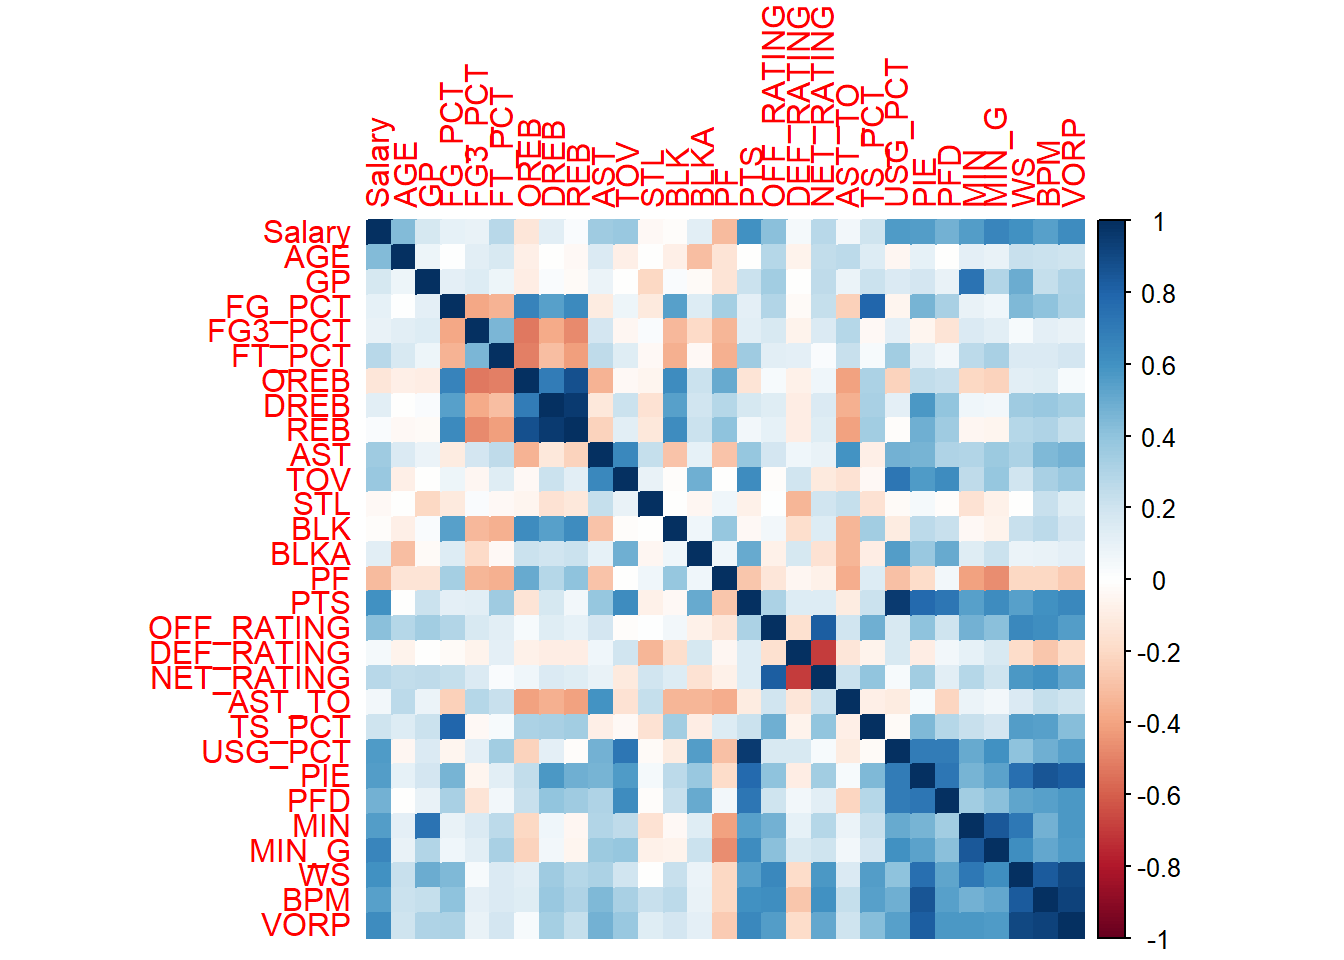
\includegraphics[width=0.8\linewidth]{Report_files/figure-latex/corrplot-independent-variables-1} 

}

\caption{Correlation plot of the independent numeric variables \label{fig:corrplot-independent-variables}}\label{fig:corrplot-independent-variables}
\end{figure}

Different correlations between the variables emerge from the
\texttt{corrplot}. With regard to the variable Salary, it is interesting
to notice that Salary is positively correlated with PTS (points) and
with advanced stats like USG\_PCT, BPM and VORP: all of these variables
are related to players' shots and point contribution. For what concerns
the other variables, there are some obvious correlations: for instance,
between variables MIN (total minutes played during the regular season)
and MIN\_G (minutes played per game) and between variables REB, OREB and
DREB (indicating rebounds, with the relation REB = OREB + DREB).
Additionally, we expected the positive correlation between BPM and VORP
because are both related to players point estimation.

A strong positive correlation emerges between PTS and USG\_PCT (the
percentage of team plays used by a player when they are on the floor.
Formula: (FGA + Possession Ending FTA + TO) / POSS). Thus, players with
a high USG\_PCT often make the last play in an offensive possession (a
shot, a free throw or a turnover): it is straightforward that if a
player often ends the offensive possession of his team, he has more
opportunities to score points.

For what concerns the negative correlations, the most interesting are
the ones between rebounds variables (OREB, DREB, REB), FT\_PCT and
FG3\_PCT. Players that grab a lot of rebounds are usually the tallest
ones and these players are not great free throws shooters or 3 point
shooters (on average).

\hypertarget{data-analysis-and-interpretation}{%
\section{Data analysis and
interpretation}\label{data-analysis-and-interpretation}}

\hypertarget{models}{%
\subsection{Models}\label{models}}

We started creating a complete linear regression model that includes all
the predictors.

\begin{verbatim}
## 
## Call:
## lm(formula = Salary ~ +., data = fd_numeric)
## 
## Residuals:
##       Min        1Q    Median        3Q       Max 
## -18450260  -4028989    276645   4003025  20712902 
## 
## Coefficients:
##               Estimate Std. Error t value Pr(>|t|)    
## (Intercept)  -12550803   28966256  -0.433   0.6651    
## AGE            1057586      93293  11.336   <2e-16 ***
## GP              -21024     118116  -0.178   0.8588    
## FG_PCT        35836089   19086013   1.878   0.0613 .  
## FG3_PCT         -56045    4195524  -0.013   0.9893    
## FT_PCT          975535    6135667   0.159   0.8738    
## OREB           4054377    6865112   0.591   0.5552    
## DREB           4473997    6846450   0.653   0.5139    
## REB           -4315225    6838752  -0.631   0.5285    
## AST             -98527     667680  -0.148   0.8828    
## TOV            2003183    1516145   1.321   0.1873    
## STL             -69046     985541  -0.070   0.9442    
## BLK             601287     664109   0.905   0.3659    
## BLKA          -2253383    1230646  -1.831   0.0680 .  
## PF             -616626     640191  -0.963   0.3362    
## PTS            1117890     623630   1.793   0.0740 .  
## OFF_RATING    16646653    6955245   2.393   0.0172 *  
## DEF_RATING   -16681974    6953008  -2.399   0.0170 *  
## NET_RATING   -16610236    6957987  -2.387   0.0175 *  
## AST_TO         -252115     978605  -0.258   0.7969    
## TS_PCT       -63710004   30332753  -2.100   0.0365 *  
## USG_PCT      -40539821   73391644  -0.552   0.5811    
## PIE         -131534170  115933751  -1.135   0.2574    
## PFD             101829     397847   0.256   0.7981    
## MIN              -4774       4689  -1.018   0.3094    
## MIN_G           696311     299872   2.322   0.0208 *  
## WS             1845668     740418   2.493   0.0132 *  
## BPM            -391702     764769  -0.512   0.6089    
## VORP            663105    1436430   0.462   0.6446    
## ---
## Signif. codes:  0 '***' 0.001 '**' 0.01 '*' 0.05 '.' 0.1 ' ' 1
## 
## Residual standard error: 6712000 on 331 degrees of freedom
## Multiple R-squared:  0.7081, Adjusted R-squared:  0.6834 
## F-statistic: 28.67 on 28 and 331 DF,  p-value: < 2.2e-16
\end{verbatim}

\begin{figure}

{\centering 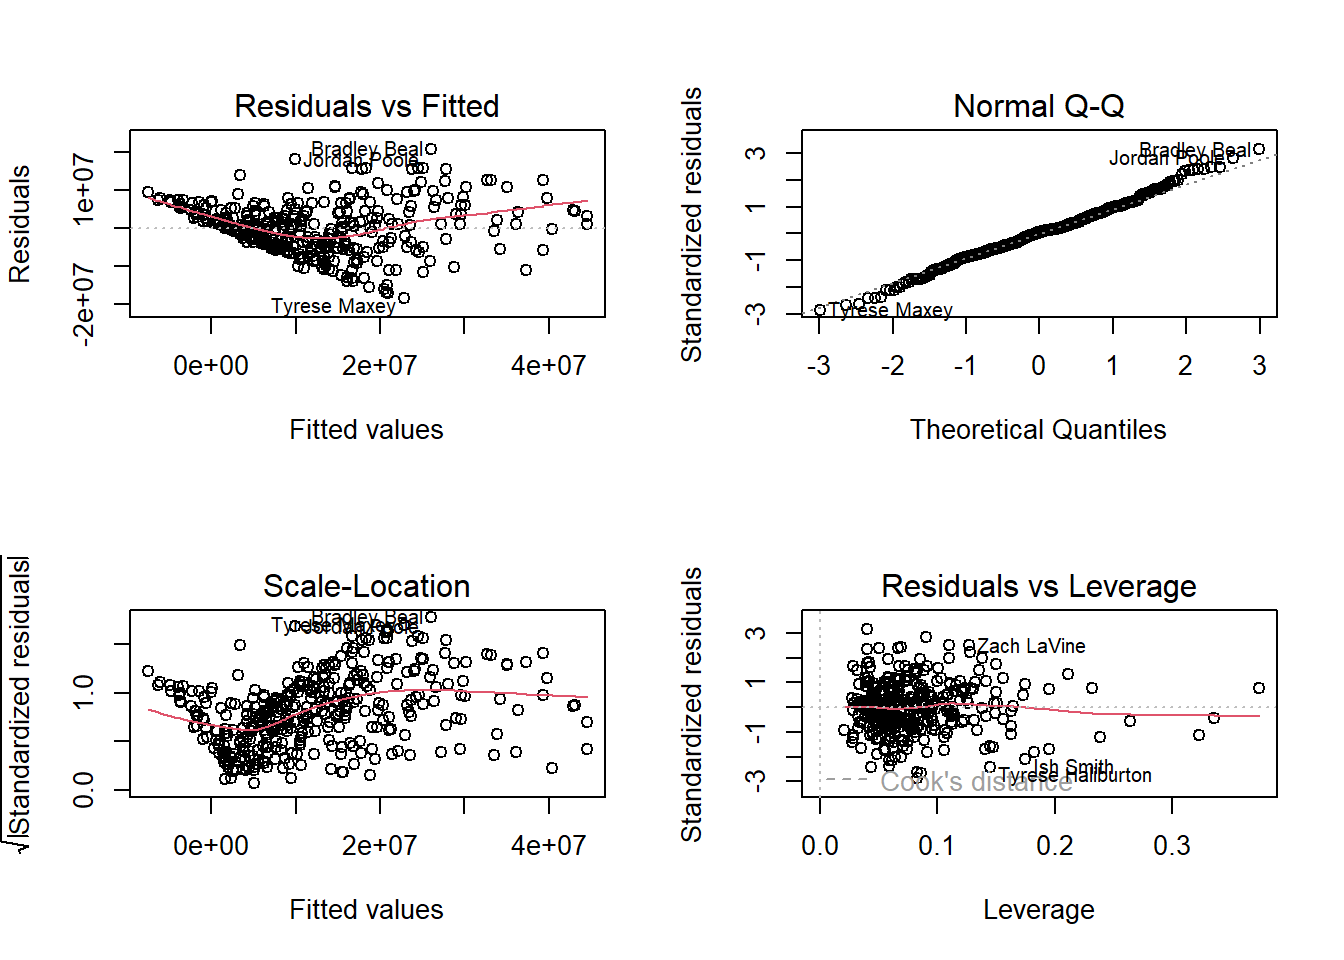
\includegraphics[width=0.9\linewidth]{Report_files/figure-latex/linear-regression-model-1} 

}

\caption{Residuals plot of the complete linear model \label{fig:linear-regression-model}}\label{fig:linear-regression-model}
\end{figure}

\begin{verbatim}
## [1] "MSE of the complete linear model =  4.142347e+13"
\end{verbatim}

The complete model has a good R-squared of 0.7081 and a MSE of 4.14e+13.
It emerges that many variables are not significant in determining the
response. Through the residual analysis (Figure
\ref{fig:linear-regression-model}) it is noticeable that the
relationship between fitted values and residuals is not exactly linear
(first graph). Additionally, in the third graph the points are not are
included in a band of constant amplitude parallel to the x-axis, hence
the omoschedasticity assumption can be doubted.

We tried to apply a logarithmic transformation to the dependent
variable: the model showed a lower R-squared (0.6516) and a slightly
higher MSE (4.70e+13). On the other hand, the first graph showed a more
linear relationship and the third graph allowed to infer a more constant
variance in the error terms. Nevertheless, the deterioration in
performance suggests that the logarithmic transformation is not the most
suitable.

\begin{verbatim}
## 
## Call:
## lm(formula = sqrt(Salary) ~ ., data = fd_numeric)
## 
## Residuals:
##      Min       1Q   Median       3Q      Max 
## -2404.66  -480.54   -33.85   587.26  2307.27 
## 
## Coefficients:
##               Estimate Std. Error t value Pr(>|t|)    
## (Intercept) -1.488e+03  3.826e+03  -0.389   0.6976    
## AGE          1.470e+02  1.232e+01  11.934   <2e-16 ***
## GP          -4.891e+00  1.560e+01  -0.314   0.7541    
## FG_PCT       4.886e+03  2.521e+03   1.938   0.0534 .  
## FG3_PCT     -5.984e+01  5.541e+02  -0.108   0.9141    
## FT_PCT      -4.782e+01  8.104e+02  -0.059   0.9530    
## OREB         5.098e+02  9.067e+02   0.562   0.5743    
## DREB         5.872e+02  9.042e+02   0.649   0.5165    
## REB         -5.355e+02  9.032e+02  -0.593   0.5537    
## AST          2.237e+01  8.818e+01   0.254   0.7999    
## TOV          1.482e+02  2.002e+02   0.740   0.4598    
## STL          3.458e+01  1.302e+02   0.266   0.7907    
## BLK          1.075e+02  8.771e+01   1.226   0.2212    
## BLKA        -3.018e+02  1.625e+02  -1.857   0.0642 .  
## PF          -7.267e+01  8.455e+01  -0.859   0.3907    
## PTS          1.428e+02  8.237e+01   1.733   0.0840 .  
## OFF_RATING   2.273e+03  9.186e+02   2.474   0.0139 *  
## DEF_RATING  -2.268e+03  9.183e+02  -2.470   0.0140 *  
## NET_RATING  -2.268e+03  9.190e+02  -2.468   0.0141 *  
## AST_TO      -4.468e+01  1.292e+02  -0.346   0.7298    
## TS_PCT      -8.454e+03  4.006e+03  -2.110   0.0356 *  
## USG_PCT     -3.479e+03  9.693e+03  -0.359   0.7199    
## PIE         -2.165e+04  1.531e+04  -1.414   0.1583    
## PFD          2.130e+01  5.255e+01   0.405   0.6854    
## MIN         -3.237e-01  6.193e-01  -0.523   0.6015    
## MIN_G        9.071e+01  3.961e+01   2.290   0.0226 *  
## WS           2.349e+02  9.779e+01   2.402   0.0169 *  
## BPM          7.005e+00  1.010e+02   0.069   0.9448    
## VORP        -8.645e+01  1.897e+02  -0.456   0.6489    
## ---
## Signif. codes:  0 '***' 0.001 '**' 0.01 '*' 0.05 '.' 0.1 ' ' 1
## 
## Residual standard error: 886.5 on 331 degrees of freedom
## Multiple R-squared:  0.7089, Adjusted R-squared:  0.6842 
## F-statistic: 28.78 on 28 and 331 DF,  p-value: < 2.2e-16
\end{verbatim}

\begin{figure}

{\centering 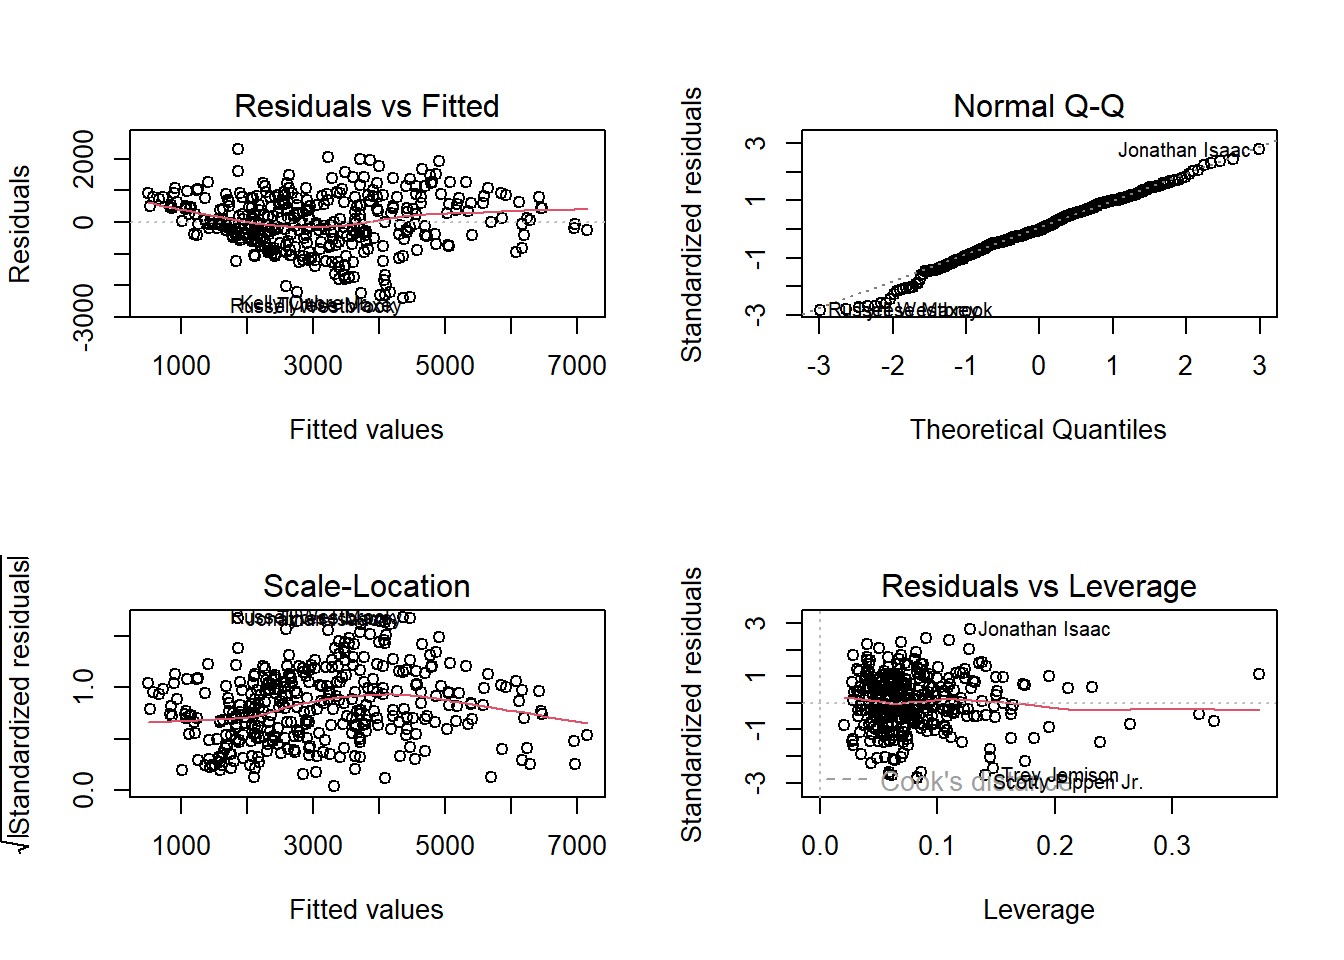
\includegraphics[width=0.9\linewidth]{Report_files/figure-latex/square-root-transformation-1} 

}

\caption{Residuals plot of the complete linear model with square rooted Salary \label{fig:square-root-transformation}}\label{fig:square-root-transformation}
\end{figure}

\begin{verbatim}
## [1] "MSE of the complete linear model with square rooted Salary =  3.607895e+13"
\end{verbatim}

For this reason, we chose to use the square root. The performance was
better compared to the other two models: 0.7089 R-Squared, 3.607895e+13
MSE. Moreover, as can be seen in the Figure
\ref{fig:square-root-transformation}, the relationship is more linear
and the variance in the error terms is more constant compared to the
model without transformations.

By the way, in both models many variables are not significant in
determining the response: for this reason, to avoid a model that is
unnecessary complex, we performed a variable selection. A square root
transformation of the dependent variable Salary will be applied because
it improves the performance of the complete model, it makes the salaries
distribution closer to normal, it improves the linearity of the model
and it reduces residuals eteroschedasticity.

\hypertarget{variable-selection}{%
\subsubsection{Variable selection}\label{variable-selection}}

We selected a subset of relevant features starting from the predictors
used in the complete model in order to have a simpler model that is
easier to interpret, without redundant variables and less prone to
overfitting. To do so, we used the \texttt{regsubsets} function which
performs best subset selection by identifying the best model that
contains a given number of predictors, according to the RSS metric. We
set the function to return results up to the best 28-variables model.

To find the best balance between model simplicity and precision, we
evaluated the number of parameters to be included in the model through
Mallow's Cp, BIC and Adjusted R-squared.

\begin{figure}

{\centering 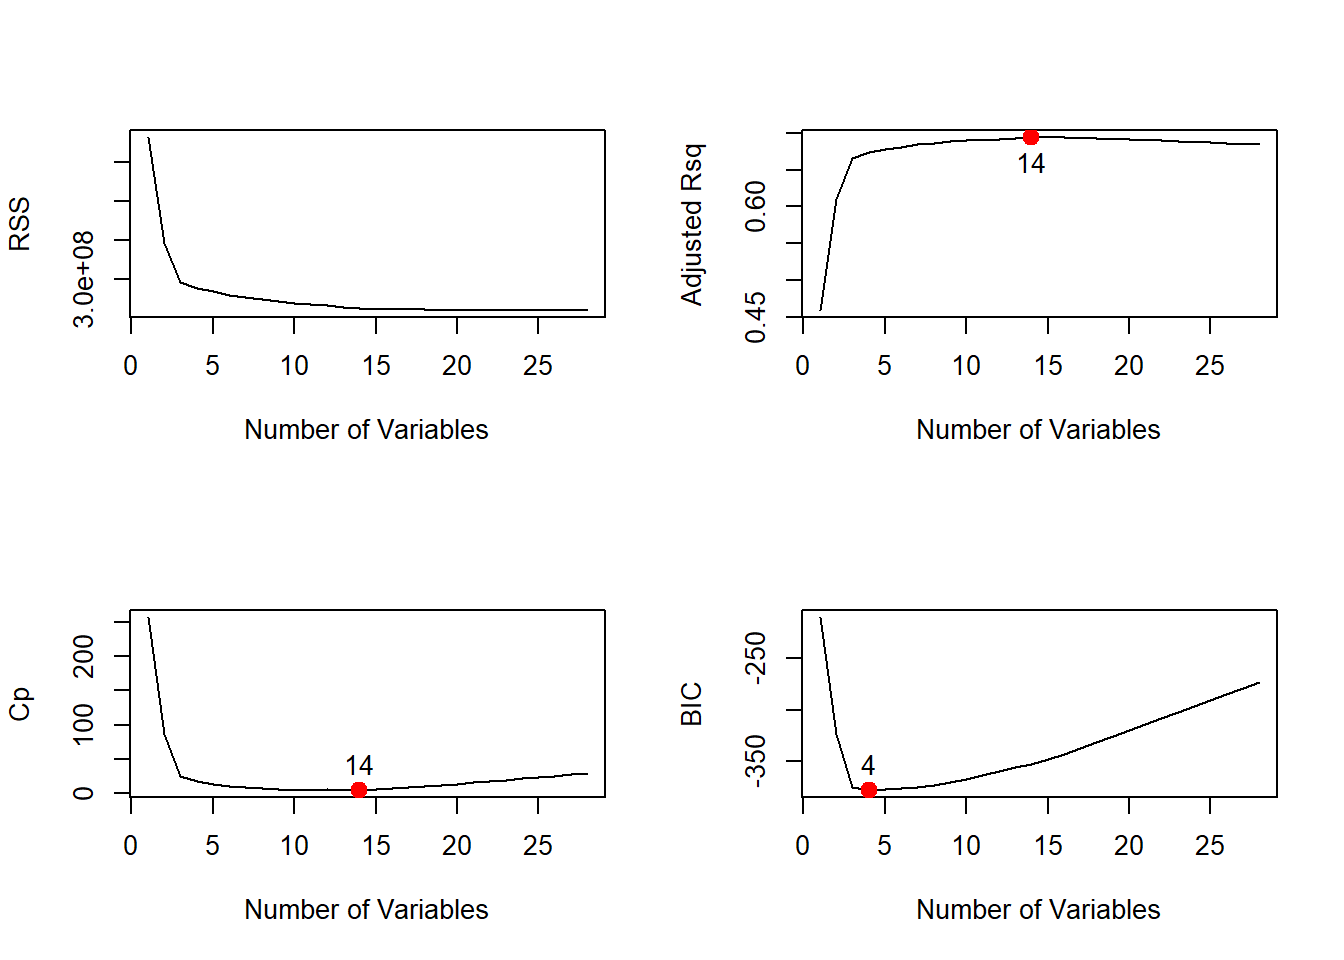
\includegraphics[width=0.9\linewidth]{Report_files/figure-latex/parameters-selection-1} 

}

\caption{Evaluation of the number of parameters through RSS, Adjusted R-squared, Mallow's Cp and BIC \label{fig:parameters-selection}}\label{fig:parameters-selection}
\end{figure}

Considering Mallow's Cp, the best number of parameters for our model is
14. This result can be seen in the Figure
\ref{fig:parameters-selection}. We obtained the list of parameters from
the \texttt{regsubset} function to get the best model with 14
parameters.

\begin{Shaded}
\begin{Highlighting}[]
\FunctionTok{summary}\NormalTok{(lm.ess)}
\end{Highlighting}
\end{Shaded}

\begin{verbatim}
## 
## Call:
## lm(formula = selected.formula, data = df)
## 
## Residuals:
##      Min       1Q   Median       3Q      Max 
## -2481.69  -500.09   -10.46   594.24  2324.15 
## 
## Coefficients:
##               Estimate Std. Error t value Pr(>|t|)    
## (Intercept)  -2377.429   2272.271  -1.046 0.296165    
## AGE            145.703     11.866  12.279  < 2e-16 ***
## GP             -10.827      4.030  -2.687 0.007564 ** 
## FG_PCT        4709.742   1617.341   2.912 0.003825 ** 
## TOV            124.049     72.057   1.722 0.086051 .  
## BLK            106.418     69.734   1.526 0.127914    
## BLKA          -292.699    148.935  -1.965 0.050183 .  
## PTS            105.824     16.299   6.493 2.94e-10 ***
## OFF_RATING    2363.880    880.378   2.685 0.007602 ** 
## DEF_RATING   -2354.167    880.651  -2.673 0.007870 ** 
## NET_RATING   -2358.170    880.370  -2.679 0.007747 ** 
## TS_PCT       -7719.606   2035.977  -3.792 0.000177 ***
## PIE         -15116.488   4308.295  -3.509 0.000510 ***
## MIN_G           77.230      9.796   7.884 4.21e-14 ***
## WS             178.374     43.211   4.128 4.59e-05 ***
## ---
## Signif. codes:  0 '***' 0.001 '**' 0.01 '*' 0.05 '.' 0.1 ' ' 1
## 
## Residual standard error: 872.4 on 345 degrees of freedom
## Multiple R-squared:  0.7061, Adjusted R-squared:  0.6942 
## F-statistic: 59.21 on 14 and 345 DF,  p-value: < 2.2e-16
\end{verbatim}

The reduced model shows a 0.7061 R-squared, that indicates a good fit.

Different variables are strongly significant:

\begin{itemize}
\item
  \textbf{AGE}: the positive coefficient associated to the variable
  shows that older players earn, on average, more than young ones. This
  makes sense since the youngest players in the league, rookies (first
  year in NBA) and sophomores (second year in NBA), usually earn less in
  the first years due to particular specifications in their contracts.
  However, there are also many veterans that sign for very low salaries
  in order to play with better teams and thus have a chance of winning
  the title.
\item
  \textbf{PTS}: this is quite straightforward. Players who score more
  points, on average, have higher salaries.
\item
  \textbf{TS\_PCT}: for what concerns true shooting percentage, the
  situation is peculiar. TS\_PCT weights a player's shooting percentages
  based on the shot type (3-pointer, 2 pointer or free throw). The
  negative coefficient seems counter intuitive: a better TS\_PCT
  reflects, on average, a lower salary. A possible explanation is that
  this metric is high for two players categories. The first one is
  composed by tall players who take most of their shots near the basket,
  thus getting a high percentage. The second category is composed by
  3-point shooting specialists, because the weight for a 3 point shoot
  is higher for the metric. These players are crucial into a team, but
  we can say that they often have a limited role: the former have to
  score mostly near the basket, the latter from behind the 3-point line.
  Consequently, it makes sense if the model assigns a lower salary for
  players with a limited role. Additionally, shooting percentages are
  also high for players that shoot only few shots in a game; it is
  reasonable to think that scoring only few shots it's not enough to
  earn a high salary. Moreover, it is important to highlight that the
  best players (the ones that should earn more) attract more attention
  from opposing defenders, so it is normal that they have more
  fluctuating shooting percentages than previous mentioned specialists.
\item
  \textbf{MIN\_G}: players that play on average more minutes in a game
  earn, on average, a higher salary.
\item
  \textbf{PIE}: for what concerns PIE, we did not expect a highly
  negative coefficient. This metric measures the impact of a player in a
  single match. The negative sign has different possible explanations:
  projecting PIE per 48 minutes inflates the metric for players who have
  a high impact on the game but few minutes played. It considers a lot
  of stats, even stats that seem to be not significant in determining
  salary; PIE difference between high salary players and low salary ones
  is not proportional to the differences in salaries. It is always
  difficult consider defensive contribution with this kind of metric and
  it is reasonable to think that defensive contribution plays an
  important role in determining a players salary. Furthermore, PIE does
  not consider aspects like leadership and IQ that, as defensive
  contribution, will certainly have an impact on the salaries.
\item
  \textbf{WS}: the variable Win Shares attempts measures each player
  contribution for team success. Consequently, we were expecting that
  higher values of WS have a positive impact on the Salary.
\end{itemize}

The variable FG\_PCT is less significant than TS\_PCT, but the
coefficient here is positive. Both the stats measure shooting
percentages, but FG\_PCT does not weight shots and does not consider
free throws. In this way, the previous mentioned effect on 3 point
shooting specialists is reduced. It is possible to infer that FG\_PCT
represents better, within this model, the positive impact of good
shooting percentages on wages.

The variables OFF\_RATING, DEF\_RATING, NET\_RATING, GP and FG\_PCT have
a level of significance between 0.001 and 0.01. The positive sign of
OFF\_RATING and FG\_PCT coefficients and the negative sign of
DEF\_RATING coefficient are in line with what we expected. OFF\_RATING
(DEF\_RATING) represents the points scored (conceded) by the team when
the player is playing, WS measures the player contribution to the team
wins. We didn't expected negative signs for NET\_RATING (OFF\_RATING -
DEF\_RATING) and GP (slightly negative)

Beyond all the possible explanations, these unexpected negative signs
likely depend from other variables not included in the model.

\hypertarget{correlation-between-dependent-variables}{%
\paragraph{Correlation between dependent
variables}\label{correlation-between-dependent-variables}}

\begin{figure}

{\centering 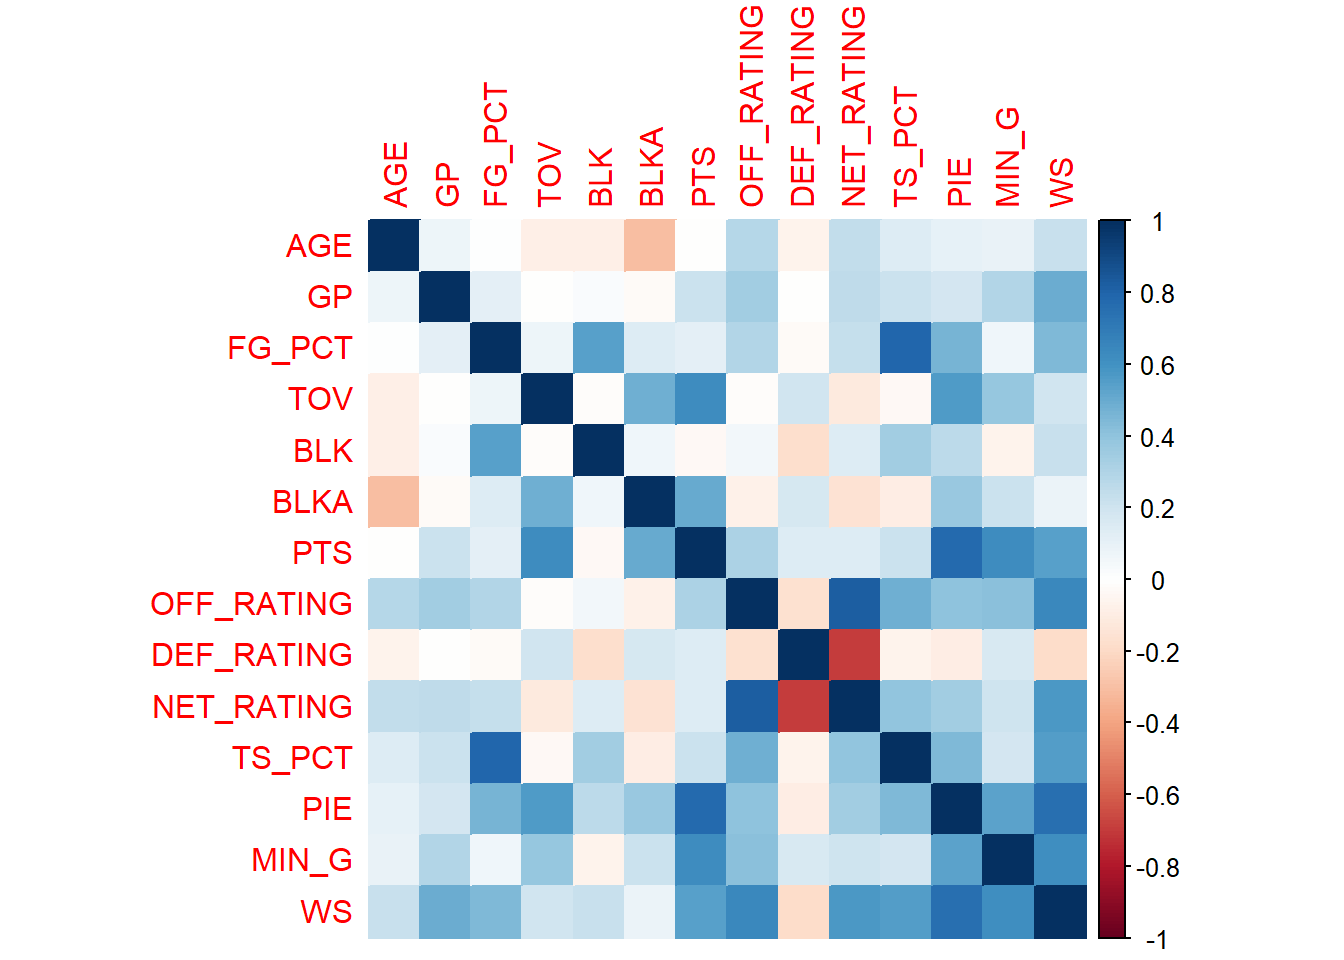
\includegraphics[width=0.8\linewidth]{Report_files/figure-latex/correlation-independent-variables-1} 

}

\caption{Correlation between dependent variables of the reduced model \label{fig:correlation-independent-variables}}\label{fig:correlation-independent-variables}
\end{figure}

It can be seen in the Figure \ref{fig:correlation-independent-variables}
that there are, also in this case, different correlations between the
dependent variables.

\hypertarget{residual-analysis}{%
\paragraph{Residual analysis}\label{residual-analysis}}

\begin{figure}

{\centering 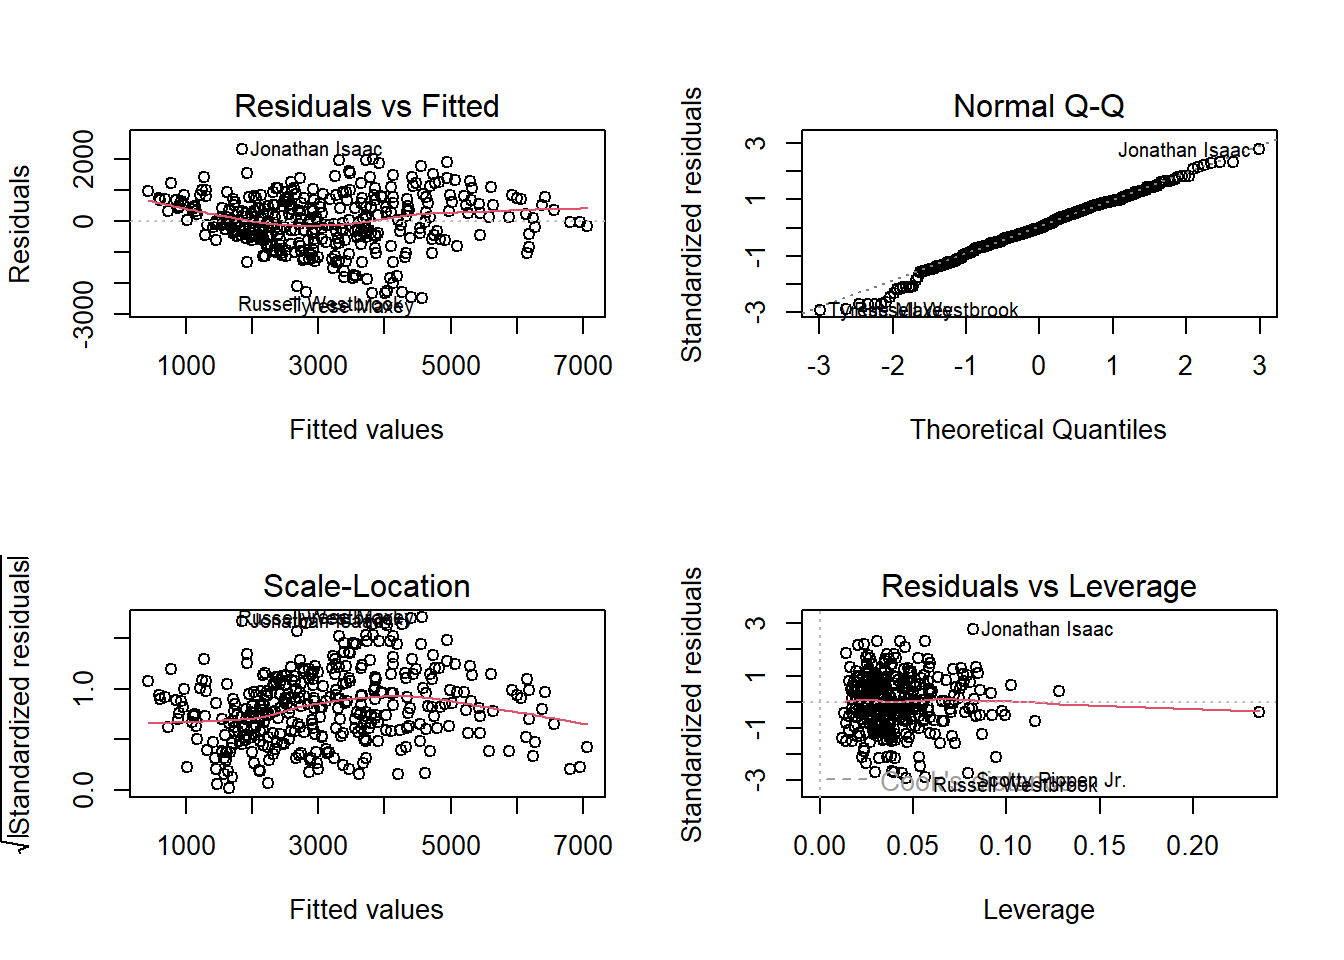
\includegraphics[width=0.9\linewidth]{Report_files/figure-latex/residual-analysis-ess-1} 

}

\caption{Residual plot of the reduced model with 14 covariates \label{fig:residual-analysis-ess}}\label{fig:residual-analysis-ess}
\end{figure}

From what can be seen in the Figure \ref{fig:residual-analysis-ess}, the
assumptions of the linear model seem to be fulfilled. There are some
players who are outliers in each graph.

\hypertarget{mse}{%
\paragraph{MSE}\label{mse}}

\begin{verbatim}
## [1] "MSE of the reduced linear model with square root Salary =  5.319559e+11"
\end{verbatim}

\begin{verbatim}
## [1] "Square rooted MSE of the reduced linear model with square root Salary =  7.293531e+05"
\end{verbatim}

The reduced model has a very good MSE calculated on the whole model:
5.319559e+11. In order to compare different models, we divided the
dataset into train and test. Once fitted the model on the training set,
we evaluated the performance on the test set to avoid overfitting.

\begin{verbatim}
## [1] "Estimated test MSE =  4.448972e+13"
\end{verbatim}

\begin{verbatim}
## [1] "Square root of the estimated test MSE =  6.670061e+06"
\end{verbatim}

The estimated MSE on the test set is 4.449e+13. We will use this value
to compare the model with the next ones.

\hypertarget{comparison-between-real-salaries-and-salaries-prediction}{%
\paragraph{Comparison between real salaries and salaries
prediction}\label{comparison-between-real-salaries-and-salaries-prediction}}

\begin{longtable}[]{@{}lrrr@{}}
\caption{Ten most overpaid players according to the reduced
model}\tabularnewline
\toprule()
& Salary & Predicted salary & Difference \\
\midrule()
\endfirsthead
\toprule()
& Salary & Predicted salary & Difference \\
\midrule()
\endhead
Bradley Beal & 46741590 & 24358643 & 22382947 \\
Zach LaVine & 40064220 & 20681956 & 19382264 \\
Darius Garland & 34005250 & 14635007 & 19370243 \\
Deandre Ayton & 32459438 & 13809140 & 18650298 \\
Michael Porter Jr. & 33386850 & 15306816 & 18080034 \\
Jordan Poole & 27955357 & 11003024 & 16952333 \\
Tobias Harris & 39270150 & 22395296 & 16874854 \\
Trae Young & 40064220 & 24504123 & 15560097 \\
Fred VanVleet & 40806300 & 25628038 & 15178262 \\
Klay Thompson & 43219440 & 28056247 & 15163193 \\
\bottomrule()
\end{longtable}

\begin{longtable}[]{@{}lrrr@{}}
\caption{Ten most underpaid players according to the reduced
model}\tabularnewline
\toprule()
& Salary & Predicted salary & Difference \\
\midrule()
\endfirsthead
\toprule()
& Salary & Predicted salary & Difference \\
\midrule()
\endhead
Tyrese Maxey & 4343920 & 20847446 & 16503526 \\
Russell Westbrook & 3835738 & 19419261 & 15583523 \\
Desmond Bane & 3845083 & 18158172 & 14313089 \\
Kelly Oubre Jr. & 2891467 & 16072226 & 13180759 \\
Eric Gordon & 3196448 & 16357558 & 13161110 \\
Jalen Williams & 4558680 & 17084418 & 12525738 \\
Cam Thomas & 2240160 & 14547343 & 12307183 \\
Tyrese Haliburton & 5808435 & 17514933 & 11706498 \\
Reggie Jackson & 5000000 & 16679982 & 11679982 \\
Jalen Brunson & 26346666 & 37833452 & 11486786 \\
\bottomrule()
\end{longtable}

Here we have a comparison between real salaries and predicted ones. The
tables contain, respectively, the 10 most overpaid players and the 10
most underpaid players according to the model. The aim of this
comparison is to analyse the major differences between predictions and
actual salaries to understand whether, despite a big difference, the
model's predictions seem reasonable.

\textbf{MOST OVERPAID PLAYERS}

The most overpaid player results to be Bradley Beal. After some
brilliant seasons with Washington Wizards in which he was the league top
scorer, he signed in 2022 a maximum contract (251 million \$ in
5-years). In Washington he was the best player by far, his statlines in
the past years justify the huge contract. In 23-24 he was traded to
Phoenix (keeping the same contract) to play with Durant and Booker (two
superstars) in a team that was, on the paper, a contender for the title.
Beal, being no longer the first offensive option, had a quite different
statline compared to the previous years. Additionally, the whole Phoenix
Suns team disappointed the expectations. These facts are enough to
explain that Beal's 23-24 performance is not in line with his salary.

Darius Garland signed a big contract (near to the maximum) starting from
23-24 season. After showing superstar potential in 22-23, Cleveland
Cavaliers renewed his contract with an important salary increase but
Garland's performance decreased in 23-24. He is only 24, the team bet
heavily on him taking a weighted risk in order to keep with them a high
potential player. This bet didn't paid in 23-24 season.

Trae Young and Zach Lavine have superstar contracts respectively in
Atlanta and Chicago, but they are not carrying their teams as expected.
Both players could be traded during this summer.

Regarding Deandre Ayton, he was an amazing prospect but he repeatedly
failed to meet expectations at the most important moments. He signed a
big contract in 2022 but his performance were not at the same level as
the salary. He was traded to Washington (keeping the same contract) but
also this year in a different team he did not fulfil expectations.

Michael Porter Jr.~(especially the former) is a young player that in his
still short careers has not shown his full potential due to injuries.
His contract, let's say, considers his potential performance at the top
of his form.

Jordan Poole had an exploit in the previous seasons playing with a top
team, Golden State Warriors, that somehow justifies his salary. He
seemed to be ready to carry a team on his own, he was traded to
Washington but his first season was a failure.

Klay Thompson, after being a key piece in the Golden State Warriors
dinasty, suffered a serious injury few years ago. After that, he was no
longer the same player and the salary was, let's say, no longer adequate
to his performance. His contract with Golden State ended after the 23-24
season and he recently signed with Dallas Mavericks for 50 millions in 3
years, thus he will earn a salary closer (even lower) to the predicted
one.

Regarding Tobias Harris, this was the last contract year with
Philadelphia 76ers. He signed this contract in 2019, team's situation
was really different, Harris seemed to be the missing piece to build a
contender for the title. After 5 years and a lot of changes, his
situation is similar to Thompson's: salary not in line with performance.
In fact, he also signed recently with another team (Detroit Pistons) for
52 millions in 2 years, really close to the prediction.

Fred Vanvleet signed a big contract with Houston Rockets last year. The
team has a young core, they are in a rebuilding phase so for the moment
they don't have ambitions for the title. Without being a contender,
teams are less attractive for the superstars. For this reason, they
signed a really good player paying him like a superstar: the fact that
he results as really overpaid was quite predictable.

\textbf{MOST UNDERPAID PLAYERS}

Jalen Brunson has shown this year that he is one of the best players in
the NBA after being somewhat underrated in the years past. We expected
the difference between his predicted and actual salary. Very similar the
situation of Tyrese Maxey, in the last year of his rookie contract. He
has shown by his performances that he is worth much more than his salary
says.

Russell Westbrook is in the waning phase of his career. On the expiry of
his last superstar contract, no team in the league offered him a
comparable salary (he earned 47 millions in 2022). Consequently, he
accepted a 3.8 millions salary (veteran minimum contract) to play with
Los Angeles Clippers. For sure he is no longer a player worth 47
millions, but he is not worth 3.8 millions either. Our model interprets
pretty well the situation, stating that Westbrook should earn a 18.3
millions salary: not a superstar one, but not a minimum wage either.

Eric Gordon is a veteran, he signed for a very small salary with Phoenix
Suns in order to play with a contender. This move is not uncommon for
good players in the final part of their career, especially if they never
won a NBA title like Gordon. In the previous contract with Houston
Rockets Gordon earned 75.6 millions in 4 years, perfectly in line with
the prediction.

Bane, Haliburton, Thomas and Williams have a Maxey-like situation: they
are young players which are still in their rookie contracts but they
clearly overperformed considering how much they earn. Maybe the model
over evaluates a bit Cam Thomas, because he produces really good
offensive numbers (the stats and the models capture the offensive
contribution really well, much less the defensive one) when called on
but his performance decrease when it comes to defense. Additionally, he
could improve in leadership and understanding of the game.

Oubre's last contract was 30 millions in 2 years with Phoenix Suns, so
in line with the predicted one. Last year he signed a small 2.89 million
one-year contract with Philadelphia 76ers for several reasons: injury
history, lack of performance consistency, market dynamics. Probably he
will sign a new contract soon.

Given the presence of correlations between the independent variables,
the presence of multicollinearity is likely. For this reason, we decided
to implement models that perform well when the variables are collinear
such as Ridge regression and Lasso regression. In the next paragraphs we
want to see if the performances of these models are better than that of
the models seen so far.

\hypertarget{ridge-regression}{%
\subsubsection{Ridge regression}\label{ridge-regression}}

The subset selection method uses least squares to fit a linear model
with a subset of the predictors. On the other hand, ridge regression
does not select a subset of the coefficients \emph{\(\beta_j\)} of the
model, but it fits a model with all \emph{p} predictors adding a term
\(\lambda \sum^p_{j=1} \beta^2_j\). This term is called shrinkage
penalty, since it has the effect to push the coefficient estimates
towards zero. Lambda (\(\lambda\)) is a tuning parameter that controls
the impact of the penalty on the estimates. In order to determine a good
value for \(\lambda\), we used a ten-fold cross-validation. We also used
a square root transformation of the dependent variable in this model
because, as mentioned before, it improves linearity, omoschedasticity,
variable's normality and it reduces the influence of outliers.

\begin{figure}

{\centering \includegraphics[width=0.9\linewidth]{Report_files/figure-latex/ridge-square-root-lambda-1} 

}

\caption{Plot of the cross-validated MSE with respect to the value of $\lambda$ in the Ridge regression model \label{fig:ridge-lambda}}\label{fig:ridge-square-root-lambda}
\end{figure}

\begin{verbatim}
## [1] "The best lambda is =  153"
## [1] "The estimated test MSE with the best lambda is =  4.867254e+13"
\end{verbatim}

In the plot of the Figure \ref{fig:ridge-lambda} the red dotted line
represents the cross-validation curve with upper and lower standard
deviation curves along the \(\lambda\) sequence. We chose the value of
\(\lambda\) (153) that gives minimum mean cross-validated error. The
mean squared error on the test set is 4.867e+13. Applying the square
root transformation of the dependent variable Salary does not influence
the \(\lambda\) value returned by the k-fold cross-validation since it
is a monotonic transformation and it does not changes the relative
ranking of \(\lambda\).

\begin{figure}

{\centering \includegraphics[width=0.9\linewidth]{Report_files/figure-latex/ridge-plot-1} 

}

\caption{Plot of the values of the parameters with respect to $\lambda$ in the Ridge regression model \label{fig:ridge-plot}}\label{fig:ridge-plot}
\end{figure}

The final model was fitted with the best \(\lambda\) on all data. The
trace plot, in the Figure \ref{fig:ridge-plot}, shows how the
coefficients change if \(\lambda\) increases.

\begin{verbatim}
## [1] "R-squared =  0.7175"
\end{verbatim}

\begin{verbatim}
## [1] "MSE on the whole dataset =  4.008264e+13"
\end{verbatim}

Once fitted the model on all data with the best lambda, we evaluated the
performance on the whole dataset. The 0.72 R-squared highlights a very
good fit; also the 4.008e+13 MSE is a good result.

By the way, considering the MSE on the test set, 4.867e+13, the Ridge
regression is outperformed by the model obtained with the subset
selection (4.449e+13).

The final step is the comparison between real salaries and predicted
ones.

\begin{longtable}[]{@{}lrrr@{}}
\caption{Ten most overpaid players according to the Ridge regression
model}\tabularnewline
\toprule()
& Salary & Predicted salary & Difference \\
\midrule()
\endfirsthead
\toprule()
& Salary & Predicted salary & Difference \\
\midrule()
\endhead
Bradley Beal & 46741590 & 21040330 & 25701260 \\
Zach LaVine & 40064220 & 19257941 & 20806279 \\
Darius Garland & 34005250 & 14533439 & 19471811 \\
Deandre Ayton & 32459438 & 13218585 & 19240853 \\
Klay Thompson & 43219440 & 24705388 & 18514052 \\
Michael Porter Jr. & 33386850 & 15122623 & 18264227 \\
Jordan Poole & 27955357 & 10304747 & 17650610 \\
Tobias Harris & 39270150 & 21815514 & 17454636 \\
Fred VanVleet & 40806300 & 24004172 & 16802128 \\
Gordon Hayward & 31500000 & 16032599 & 15467401 \\
\bottomrule()
\end{longtable}

\begin{longtable}[]{@{}lrrr@{}}
\caption{Ten most underpaid players according to the Ridge regression
model}\tabularnewline
\toprule()
& Salary & Predicted salary & Difference \\
\midrule()
\endfirsthead
\toprule()
& Salary & Predicted salary & Difference \\
\midrule()
\endhead
Tyrese Maxey & 4343920 & 21966393 & 17622473 \\
Eric Gordon & 3196448 & 17996224 & 14799776 \\
Russell Westbrook & 3835738 & 18547948 & 14712210 \\
Tyrese Haliburton & 5808435 & 18576500 & 12768065 \\
Desmond Bane & 3845083 & 16605443 & 12760360 \\
Kelly Oubre Jr. & 2891467 & 15142953 & 12251486 \\
Cam Thomas & 2240160 & 14488545 & 12248385 \\
Alperen Sengun & 3536280 & 15676549 & 12140269 \\
Jalen Williams & 4558680 & 15011822 & 10453142 \\
Jalen Brunson & 26346666 & 36674733 & 10328067 \\
\bottomrule()
\end{longtable}

\textbf{MOST OVERPAID PLAYERS}

9 out of 10 players in this tier are the same as those classified as
overpaid in the previous model. Also the differences between predicted
salary and actual salary are quite similar.

\textbf{MOST UNDERPAID PLAYERS}

The same can be said for the most underpaid players: 9 out of 10 are the
same as those found in the previous model.

All in all, Ridge regression has shown satisfactory performances,
slightly improving the R-squared of the reduced model from 0.7061 to
0.7175. This result was quite expected since Ridge considers many more
predictors. For what concerns the MSE calculated on both the whole
dataset and the test set, the reduced model outperforms the Ridge
regression. Consequently, we can say that the reduced model is better in
terms of precision and parsimony.

\hypertarget{lasso-regression}{%
\subsubsection{Lasso regression}\label{lasso-regression}}

A disadvantage of ridge regression is that, unlike subset selection, it
includes all \emph{p} predictors in the final model. Also lasso
regression shrinks the coefficients estimates towards zero but it has an
absolute value shrinkage penalty instead of a quadratic one:
\(\lambda \sum^p_{j=1} |\beta_j|\). When \(\lambda\) is sufficiently
large, some coefficient estimates become exactly equal to zero. Hence,
like best subset selection, lasso performs a variable selection. As done
with the ridge, we used a root square transformation of the Salary
variable.

\begin{figure}

{\centering \includegraphics[width=0.9\linewidth]{Report_files/figure-latex/lasso-lambda-1} 

}

\caption{Plot of the cross-validated MSE with respect to the value of $\lambda$ in the Lasso regression model \label{fig:lasso-lambda}}\label{fig:lasso-lambda}
\end{figure}

\begin{verbatim}
## [1] "The best lambda is =  49"
## [1] "The estimated test MSE with the best lambda is =  4.796933e+13"
\end{verbatim}

\begin{figure}

{\centering \includegraphics[width=0.9\linewidth]{Report_files/figure-latex/lasso-plot-1} 

}

\caption{Plot of the values of the parameters with respect to $\lambda$ in the Lasso regression model \label{fig:lasso-plot}}\label{fig:lasso-plot}
\end{figure}

We followed the same procedure of the Ridge regression and the results
can be seen in the Figures \ref{fig:lasso-lambda} and
\ref{fig:lasso-plot}. The best \(\lambda\) value is 49 and the model
contains 9 variables. Among them, AGE, PTS, MIN\_G and WS that were
strongly significant also in the best subset selection model.

\begin{verbatim}
## [1] "R-squared =  0.7041"
\end{verbatim}

\begin{verbatim}
## [1] "MSE =  4.198851e+13"
\end{verbatim}

Once fitted the model on all data with the best \(\lambda\), we
evaluated the performances. The R-squared is 0.704, in line with the
other models. The Mean squared error calculated on the whole dataset is
slightly higher compared to the Ridge one, 4.198e+13 against 4.008e+13.
For what concerns the MSE calculated on the test set, it is 4.796e+13,
higher with respect to the reduced model (4.449e+13) but slightly lower
than that of the Ridge regression (4.867e+13).

\begin{longtable}[]{@{}lrrr@{}}
\caption{Ten most overpaid players according to the Lasso regression
model}\tabularnewline
\toprule()
& Salary & Predicted salary & Difference \\
\midrule()
\endfirsthead
\toprule()
& Salary & Predicted salary & Difference \\
\midrule()
\endhead
Bradley Beal & 46741590 & 20983050 & 25758540 \\
Zach LaVine & 40064220 & 20410086 & 19654134 \\
Klay Thompson & 43219440 & 23767204 & 19452236 \\
Darius Garland & 34005250 & 14576770 & 19428480 \\
Michael Porter Jr. & 33386850 & 14520473 & 18866377 \\
Deandre Ayton & 32459438 & 14321490 & 18137948 \\
Trae Young & 40064220 & 22389415 & 17674805 \\
Jordan Poole & 27955357 & 11410551 & 16544806 \\
Tobias Harris & 39270150 & 22738473 & 16531677 \\
Fred VanVleet & 40806300 & 24375929 & 16430371 \\
\bottomrule()
\end{longtable}

\begin{longtable}[]{@{}lrrr@{}}
\caption{Ten most underpaid players according to the Lasso regression
model}\tabularnewline
\toprule()
& Salary & Predicted salary & Difference \\
\midrule()
\endfirsthead
\toprule()
& Salary & Predicted salary & Difference \\
\midrule()
\endhead
Tyrese Maxey & 4343920 & 21383862 & 17039942 \\
Eric Gordon & 3196448 & 18287738 & 15091290 \\
Desmond Bane & 3845083 & 18755171 & 14910088 \\
Russell Westbrook & 3835738 & 18375701 & 14539963 \\
Kelly Oubre Jr. & 2891467 & 15859036 & 12967569 \\
Cam Thomas & 2240160 & 14364829 & 12124669 \\
Alperen Sengun & 3536280 & 15623299 & 12087019 \\
Tyrese Haliburton & 5808435 & 17281441 & 11473006 \\
Miles Bridges & 7921300 & 19164775 & 11243475 \\
Kevin Love & 3835738 & 14628749 & 10793011 \\
\bottomrule()
\end{longtable}

\textbf{MOST OVERPAID PLAYERS}

It is interesting to note that 9 out of 10 players in this table are the
same as in the corresponding table for ridge. Also the difference
between real salaries and predicted ones is very similar to that of the
previous model. The only change is the presence of Trae Young here (he
was one the most overpaid players in the best subset selection model)
instead of Gordon Hayward in the Ridge.

\textbf{MOST UNDERPAID PLAYERS}

Also in this case, 8 out of 10 players are the same as in the Ridge and
the differences are really small. One of the changes is the presence of
Kevin Love. As Eric Gordon, he is a veteran and he signed for a small
salary with Miami Heat.

We can state that Lasso regression has better performance compared to
Ridge regression: the R-squared and the MSE on the whole dataset are
slightly worse, but the MSE on the test set is higher. This is an
important result, especially considering that Lasso regression model is
way simpler (only 9 predictors). Placing in contrast the Lasso
regression and the reduced model it is important to consider that,
despite a higher MSE on the test, the first model is more parsimonious,
9 predictors against 14. On the other hand, the latter is more precise.

\hypertarget{salaries-analysis-by-position}{%
\subsection{Salaries analysis by
position}\label{salaries-analysis-by-position}}

In the last part of the study, we wanted to analyse salaries by grouping
players with respect to their playing positions. We considered the
classic split of centers, forwards and guards.

First of all, we wanted to check whether players earn, on average, the
same salary regardless of their role. To do so, we used the ANOVA to
compare the means of the different groups.

Secondly, we implemented different models to explore the relationship
between salaries and performance for each position. Given what emerged
from the comparison between Lasso and the reduced model, we can say that
neither model is clearly better than the other. The choice depends on
the purpose of the research. In this case, we implemented for each
position both a model built with subset selection and Lasso regression
(for a total of 6 models); here only the 3 models that best fit the data
are shown.

The objectives are:

\begin{itemize}
\item
  observe the differences between the selected predictors of the
  role-specific models among themselves and with respect to the general
  models (considering all the positions);
\item
  compare position-specific models' performances between each other and
  with the general models;
\item
  compare the predictions of the most overpaid and most underpaid
  players between position-specific and general models.
\end{itemize}

In our dataset the division was somewhat different, with 5 positions
(PG, SG, PF, SF, C). We considered point guards (PG) and shooting guards
(SG) as guards (G), power forwards (PF) and shooting forwards (SF) as
forwards (F). The centers (C) are the same.

\hypertarget{anova}{%
\subsubsection{ANOVA}\label{anova}}

The ANOVA is a hypothesis test of equal means in different groups in
which it is assumed that the variance is the same for every group; we
used it to verify if players with different roles have, on average,
different salaries. The null hypothesis states that the average salary
is the same for every position; on the other hand, the alternative
hypothesis states that at least one average salary is different.
Firstly, we tested the hypotesis of variances homogeneity with
Bartlett's test in order to see if it was possible to proceed with the
ANOVA.

\begin{Shaded}
\begin{Highlighting}[]
\FunctionTok{bartlett.test}\NormalTok{(Salary }\SpecialCharTok{\textasciitilde{}}\NormalTok{ Pos, }\AttributeTok{data =}\NormalTok{ final\_dataset)}
\end{Highlighting}
\end{Shaded}

\begin{verbatim}
## 
##  Bartlett test of homogeneity of variances
## 
## data:  Salary by Pos
## Bartlett's K-squared = 0.054132, df = 2, p-value = 0.9733
\end{verbatim}

Looking at the output, the Bartlett's K-squared was 0.054132. This small
value indicates that the difference between the observed variances
between the groups is small, as would be expected under the null
hypothesis of equality of variances. The p-value is 0.9733: considering
a significance level of 0.05, we do not have sufficient evidence to
reject the null hypothesis. Therefore, Bartlett's test shows no evidence
of unequal variances, so we can confidently proceed to the ANOVA
considering satisfied the hypothesis of homogeneity of variances.

\begin{Shaded}
\begin{Highlighting}[]
\NormalTok{aov.roles }\OtherTok{\textless{}{-}} \FunctionTok{aov}\NormalTok{(Salary }\SpecialCharTok{\textasciitilde{}}\NormalTok{ Pos, }\AttributeTok{data =}\NormalTok{ final\_dataset)}
\FunctionTok{summary}\NormalTok{(aov.roles)}
\end{Highlighting}
\end{Shaded}

\begin{verbatim}
##              Df    Sum Sq   Mean Sq F value Pr(>F)
## Pos           2 2.599e+12 1.299e+12   0.009  0.991
## Residuals   357 5.108e+16 1.431e+14
\end{verbatim}

Proceeding with ANOVA, the test statistic F results equal to 0.009. This
quantity indicates that the variability of salaries between positions is
rather small compared to the variability within positions. The p-value
is much greater than 0.05 (chosen again as level of significance), so we
don't have sufficient evidence to reject the null hypothesis. In
conclusion, there is no significant evidence to suggest that average
salaries differ significantly between different positions.

\hypertarget{centers}{%
\subsubsection{Centers}\label{centers}}

We now consider only the 67 centers present in our dataset. Starting
from the complete model (considering again the square root
transformation of Salary) we used a Lasso regression.

\begin{figure}

{\centering \includegraphics[width=0.8\linewidth]{Report_files/figure-latex/best-lambda-selection-1} 

}

\caption{Plot of the cross-validated MSE with respect to the value of $\lambda$ in the Lasso regression model for the centers}\label{fig:best-lambda-selection}
\end{figure}

\begin{verbatim}
## [1] "The best lambda is =  18"
## [1] "The estimated test MSE with the best lambda is =  5.458559e+13"
\end{verbatim}

\begin{verbatim}
## 29 x 1 sparse Matrix of class "dgCMatrix"
##                       s1
## (Intercept)  3006.660619
## AGE           113.544158
## GP              .       
## FG_PCT          .       
## FG3_PCT      -365.572419
## FT_PCT       -753.329464
## OREB            .       
## DREB          -28.826082
## REB             .       
## AST             .       
## TOV            -1.341067
## STL             .       
## BLK             .       
## BLKA         -183.407619
## PF            -26.990442
## PTS            60.066646
## OFF_RATING      .       
## DEF_RATING    -44.235200
## NET_RATING      .       
## AST_TO       -114.646897
## TS_PCT      -1027.500430
## USG_PCT         .       
## PIE             .       
## PFD            15.875756
## MIN             .       
## MIN_G         103.092503
## WS             91.701197
## BPM             .       
## VORP            .
\end{verbatim}

\begin{figure}

{\centering \includegraphics[width=0.8\linewidth]{Report_files/figure-latex/lasso-centers-coefficients-traceplot-1} 

}

\caption{Plot of the values of the parameters with respect to $\lambda$ in the Lasso regression model for the centers}\label{fig:lasso-centers-coefficients-traceplot}
\end{figure}

Once chosen the \(\lambda\) value that guarantees the lower mean
cross-validated error, we fitted the model on all data. It is
interesting that, in the particular case of centers, 13 features are
considered: the model is more complex than the general lasso model (9
predictors). Unexpectedly, despite the fact that blocks are typically a
center play, the variable BLK is excluded from the model.

\begin{verbatim}
## [1] "R-squared =  0.8217"
\end{verbatim}

\begin{verbatim}
## [1] "MSE =  2.42367e+13"
\end{verbatim}

The models' performance is really good: 0.82 R-squared and 2.423e+13
MSE. For what concerns MSE calculated on the test set, it is slightly
higher with respect to the other models: 5.458e+13 It is possible to
infer that the relationship between salaries and performance is well
represented from the model; however, it is important to consider that
the sample here is quite small, only 67 observations. For this reason,
the results must be considered carefully.

\begin{longtable}[]{@{}lrrr@{}}
\caption{Three most overpaid centers according to the Lasso regression
model}\tabularnewline
\toprule()
& Salary & Predicted salary & Difference \\
\midrule()
\endfirsthead
\toprule()
& Salary & Predicted salary & Difference \\
\midrule()
\endhead
Deandre Ayton & 32459438 & 15869488 & 16589950 \\
Kristaps Porzingis & 36016200 & 26330642 & 9685558 \\
Jaren Jackson Jr. & 27102202 & 17732344 & 9369858 \\
\bottomrule()
\end{longtable}

\begin{longtable}[]{@{}lrrr@{}}
\caption{Three most underpaid centers according to the Lasso regression
model}\tabularnewline
\toprule()
& Salary & Predicted salary & Difference \\
\midrule()
\endfirsthead
\toprule()
& Salary & Predicted salary & Difference \\
\midrule()
\endhead
Alperen Sengun & 3536280 & 17318688 & 13782408 \\
Al Horford & 10000000 & 19105610 & 9105610 \\
Nikola Vucevic & 18518519 & 26257229 & 7738710 \\
\bottomrule()
\end{longtable}

Looking at the most underpaid and most overpaid centers it emerges that
the differences between actual and predicted salaries are smaller than
in the models seen above.

\textbf{MOST OVERPAID CENTERS}

Among the overpaid centers we again find Deandre Ayton. It is quite
surprising to find Jaren Jackson Jr here. After good seasons with
Memphis Grizzlies, probably this year he suffered the drop in
performance of the entire team. He is a really good defender and an
amazing blocker: as said before, the defensive aspect of basketball is
difficult to grasp with stats (and consequently with models). Moreover,
we saw that the variable BLK is shrunk to 0 in this model, this may
partly explain why he is classified as overpaid. Regarding Porzingis, we
didn't think we would find him in this section. He was a key piece for
Boston Celtics', the team who won the title.

\textbf{MOST UNDERPAID CENTERS}

The most underpaid center results to be Alperen Sengun, a young player
still in a rookie contract. He is clearly overperforming considering how
much he earns. Al Horford is a veteran, he made an excellent
contribution to the Boston Celtics' title victory performing above the
expectations. For what concerns Nikola Vucevic, his stats are always
more than respectable. His salary is lower than the expected probably
because he seems to lack characteristics not included in the model or
generally difficult to quantify such as defense, leadership and
consistency at key moments of the season.

\hypertarget{forwards}{%
\subsubsection{Forwards}\label{forwards}}

For what concerns forwards, we have 145 observations in our dataset. In
this case, we prefer the Lasso regression model because despite more
complex, it is more accurate and makes more meaningful predictions.

\begin{figure}

{\centering \includegraphics[width=0.9\linewidth]{Report_files/figure-latex/lasso-forwards-a-1} 

}

\caption{Plot of the cross-validated MSE with respect to the value of $\lambda$ in the Lasso regression model for the forwards}\label{fig:lasso-forwards-a}
\end{figure}

\begin{verbatim}
## [1] "The best lambda is =  45"
## [1] "The estimated test MSE with the best lambda is =  4.87129e+13"
\end{verbatim}

Once found the best \(\lambda\), the model was fitted on the whole data.

\begin{verbatim}
## 29 x 1 sparse Matrix of class "dgCMatrix"
##                        s1
## (Intercept) -8238.5115564
## AGE           142.7010820
## GP              .        
## FG_PCT          .        
## FG3_PCT       817.0709843
## FT_PCT          .        
## OREB            .        
## DREB          -24.2030367
## REB             .        
## AST             .        
## TOV            71.4849990
## STL             0.1460924
## BLK            64.8173494
## BLKA            .        
## PF              .        
## PTS             .        
## OFF_RATING     29.3159113
## DEF_RATING      9.6284609
## NET_RATING      .        
## AST_TO        -80.1356585
## TS_PCT          .        
## USG_PCT      7347.9406848
## PIE             .        
## PFD            24.4890177
## MIN             .        
## MIN_G          57.3161910
## WS             32.3588419
## BPM             .        
## VORP          112.1410406
\end{verbatim}

\begin{figure}

{\centering \includegraphics[width=0.8\linewidth]{Report_files/figure-latex/lasso-forwards-1} 

}

\caption{Plot of the values of the parameters with respect to $\lambda$ in the Lasso regression model for the forwards}\label{fig:lasso-forwards}
\end{figure}

The model results simpler compared to the centers' one (11 vs 14
predictors). The variable USG\_PCT has, by far, the biggest coefficient:
according to this model, forwards who finish (with a shot, a free throw
or a turnover) most of their team's possessions, on average, earn more.
The trace plot shows how the coefficients change increasing lambda.

\begin{verbatim}
## [1] "R-squared =  0.7652"
\end{verbatim}

\begin{verbatim}
## [1] "MSE =  3.351966e+13"
\end{verbatim}

About performances, the estimated test MSE with the best lambda is
4.871e+13, in line with the models seen so far. The R-squared is quite
high, 0.76 and the MSE calculated considering every forward is
3.351e+13. We can say that the relationship between salaries and player
performance is well captured by the model.

\begin{longtable}[]{@{}lrrr@{}}
\caption{Three most overpaid forwards according to the Lasso regression
model}\tabularnewline
\toprule()
& Salary & Predicted salary & Difference \\
\midrule()
\endfirsthead
\toprule()
& Salary & Predicted salary & Difference \\
\midrule()
\endhead
Michael Porter Jr. & 33386850 & 14575242 & 18811608 \\
Tobias Harris & 39270150 & 22111611 & 17158539 \\
Klay Thompson & 43219440 & 26199144 & 17020296 \\
\bottomrule()
\end{longtable}

\begin{longtable}[]{@{}lrrr@{}}
\caption{Three most underpaid forwards according to the Lasso regression
model}\tabularnewline
\toprule()
& Salary & Predicted salary & Difference \\
\midrule()
\endfirsthead
\toprule()
& Salary & Predicted salary & Difference \\
\midrule()
\endhead
Kelly Oubre Jr. & 2891467 & 15782162 & 12890695 \\
Kevin Love & 3835738 & 15945101 & 12109363 \\
Jalen Williams & 4558680 & 15322917 & 10764237 \\
\bottomrule()
\end{longtable}

The 3 most overpaid forwards according to this model are Michael Porter
Jr, Tobias Harris and Klay Thompson. They were also among most overpaid
players in the overall lasso regression; as we said before, it is
reasonable to find these players in this tier. The same applies to Oubre
Jr and Love in terms of the 3 most underpaid forwards. Regarding
Williams, it is reasonable for him to be considered underpaid as seen
above.

\hypertarget{guards}{%
\subsubsection{Guards}\label{guards}}

Regarding guards, we consider 148 observations. Here the model obtained
through the best subset selection performs better.

\begin{figure}

{\centering \includegraphics[width=0.9\linewidth]{Report_files/figure-latex/ess-guards-1} 

}

\caption{Evaluation of the number of parameters through RSS, Adjusted R-squared, Mallow's Cp and BIC \label{fig:ess-guards}}\label{fig:ess-guards}
\end{figure}

\begin{verbatim}
## 
## Call:
## lm(formula = selected.formula, data = df)
## 
## Residuals:
##      Min       1Q   Median       3Q      Max 
## -2654.21  -564.21   -24.14   589.55  2416.84 
## 
## Coefficients:
##             Estimate Std. Error t value Pr(>|t|)    
## (Intercept) -3411.09     907.29  -3.760 0.000249 ***
## AGE           144.67      19.74   7.330 1.63e-11 ***
## FG3_PCT     -3504.98    1769.64  -1.981 0.049580 *  
## PTS            50.88      17.58   2.894 0.004415 ** 
## MIN_G         100.86      15.13   6.665 5.51e-10 ***
## BPM          -149.84      75.67  -1.980 0.049633 *  
## VORP          329.78     147.80   2.231 0.027240 *  
## ---
## Signif. codes:  0 '***' 0.001 '**' 0.01 '*' 0.05 '.' 0.1 ' ' 1
## 
## Residual standard error: 968.9 on 141 degrees of freedom
## Multiple R-squared:  0.6563, Adjusted R-squared:  0.6417 
## F-statistic: 44.88 on 6 and 141 DF,  p-value: < 2.2e-16
\end{verbatim}

According to Mallow's Cp, we chose a model with only 6 predictors
(\ref{fig:ess-guards}). This is quite surprising given that the role of
the guard is probably the most creative one in basketball: we expected a
more complex model. Nevertheless, the model fits the data quite well as
shown by the 0.66 R-squared. The variables AGE and MIN\_G are strongly
significant. The variable 3\_PCT acts in a peculiar way: the highly
negative coefficient indicates that (according to this model), on
average, guards with high percentages in 3 point shots earn less. It may
depend on the fact that many guards are 3-point specialists: thus (as
mentioned before for the variable TS\_PCT), their main contribution is
scoring behind the 3-point line. For this reason, it makes sense that
players with a limited role have a smaller salary. But again, probably
this coefficient depends from other variables that are not considered in
this model.

\begin{figure}

{\centering \includegraphics[width=0.8\linewidth]{Report_files/figure-latex/ess-guards-analysis-1} 

}

\caption{Correlation plot of the selected variables for guards \label{figess-guards-analysis}}\label{fig:ess-guards-analysis}
\end{figure}

\begin{figure}

{\centering \includegraphics[width=0.9\linewidth]{Report_files/figure-latex/res-guards-1} 

}

\caption{Residuals plot of the selected model for guards \label{fig:res-guards}}\label{fig:res-guards}
\end{figure}

Different correlations between predictors emerge from the Figure
\ref{fig:ess-guards-analysis}. Regarding the residual analysis, despite
the presence of some outliers, the linear model assumptions are
acceptably respected.

\begin{verbatim}
## [1] "MSE =  7.998341e+11"
\end{verbatim}

\begin{verbatim}
## [1] "Square rooted MSE =  8.943344e+05"
\end{verbatim}

\begin{verbatim}
## [1] "Estimated test MSE =  6.699711e+13"
\end{verbatim}

\begin{verbatim}
## [1] "Square root of the estimated test MSE =  8.185176e+06"
\end{verbatim}

Concerning performances, the estimated test MSE of 6.7e+13 is higher
compared to the previous models, but this was quite predictable due to
the low number of predictors. On the other hand, the MSE on the complete
guards dataset is really good: 7.998e+11.

\begin{longtable}[]{@{}lrrr@{}}
\caption{Three most overpaid guards according to the Lasso regression
model}\tabularnewline
\toprule()
& Salary & Predicted salary & Difference \\
\midrule()
\endfirsthead
\toprule()
& Salary & Predicted salary & Difference \\
\midrule()
\endhead
Bradley Beal & 46741590 & 19535853 & 27205737 \\
Darius Garland & 34005250 & 14145827 & 19859423 \\
Zach LaVine & 40064220 & 21087352 & 18976868 \\
\bottomrule()
\end{longtable}

\begin{longtable}[]{@{}lrrr@{}}
\caption{Three most underpaid guards according to the Lasso regression
model}\tabularnewline
\toprule()
& Salary & Predicted salary & Difference \\
\midrule()
\endfirsthead
\toprule()
& Salary & Predicted salary & Difference \\
\midrule()
\endhead
Tyrese Maxey & 4343920 & 22452630 & 18108710 \\
Eric Gordon & 3196448 & 19264808 & 16068360 \\
Russell Westbrook & 3835738 & 19570532 & 15734794 \\
\bottomrule()
\end{longtable}

We again find Beal, LaVine and Garland as the 3 most overpaid players.
Maxey, Westbrook and Gordon also here are classified among the most
underpaid players. The predictions are very similar to those of the
overall lasso regression model.

\hypertarget{conclusion}{%
\section{Conclusion}\label{conclusion}}

\hypertarget{models-performances-summary}{%
\subsection{Models performances
summary}\label{models-performances-summary}}

Summarizing, we started from a linear regression model and we applied a
square root transformation to the dependent variable Salary. Then, in
order to exclude unnecessary or redundant variables and to obtain a
simpler model, we performed a variable selection. We passed from 29 to
14 predictors with a negligible decrease in performance. However, given
the probable presence of multicollinearity between the predictors, we
implemented a Ridge regression model and a Lasso regression model. The
reduced model and the Lasso regression model outperformed Ridge
regression considering precision and parsimony. Comparing Lasso
regression and the reduced model, the former was more parsimonious but
the latter was more precise. We used Lasso regressions to analyse
centers and forwards and a model obtained through a subset selection to
analyse guards. The models for centers and forwards have shown a really
good fit with the data. Moreover, the variables considered changed both
in number and type compared to the models fitted on all players. For
what concerns guards, a very simple model emerged but with an acceptable
performance.

\hypertarget{models-limitations}{%
\subsection{Models' limitations}\label{models-limitations}}

It is necessary to remember that a lot of factors concur to determine
how much a player should earn. Regarding performances, the statistics we
used can only give a partial idea of a player's defensive contribution;
additionally, it is very difficult to understand how players perform
mentally, i.e.~to grasp characteristics such as attitude, leadership and
basketball IQ. Factors outside the basketball court also greatly
influence the determination of salaries: player's potential, player's
career, player's fit into the team, market dynamics, and so on. We
considered only a Regular Season: to have more complete models one would
have to consider more seasons and, as mentioned at the beginning, also
consider the playoffs.

\hypertarget{final-comments}{%
\subsection{Final comments}\label{final-comments}}

In the end, although their obvious limitations, some of our models
performed pretty good and provided a good basis for studying the
relationship between NBA players' salaries and performance. In
particular, Lasso regression and models obtained through a subset
selection brought valid results. As seen progressively, most of the
biggest differences between actual salaries and predicted salary were
quite reasonable.

\end{document}
